\documentclass[a4paper, 15pt]{article}
\usepackage[left=0.85in, right=0.85in, top=0.5in, bottom=0.95in]{geometry}
\usepackage[T1]{fontenc}
\usepackage[utf8]{inputenc}
\usepackage[english]{babel}

% Formattazione del testo
\usepackage{setspace}         % Setting dello spazio\begin{spacing}{0.95}
\setstretch{1.2}
\setlength{\parindent}{0pt}
\raggedbottom
\usepackage[none]{hyphenat}    % no sillabazione 
\usepackage{multicol}          % testo su più colonne
\usepackage{changepage}	       % \begin{adjustwidth}{}{}

% Matematica
\usepackage{mathtools, amssymb, amsthm, mathtools}
\usepackage{cancel}            % semplificazioni \cancel{expression}
\newtheorem*{thm}{Teorema}
\newtheorem*{en}{Enunciato}
\newtheorem*{definizione}{Definizione}
\newtheorem*{cor}{Corollario}
\DeclareMathOperator{\rk}{rk}
\DeclareMathOperator{\im}{Im}

% Simboli e Disegni
\usepackage{color}             % \textcolor{'ColorCode'}{'testo'}
\usepackage{tcolorbox}
\usepackage{graphicx, wrapfig, float}
\usepackage{tikz, circuitikz}
\usetikzlibrary{patterns, arrows, decorations.markings, arrows.meta, decorations.text}
\tikzset{immagine/.style={above right, inner sep=0pt, outer sep=0pt},
testo/.style={fill=white, align=center, fill opacity=0.6, text opacity=1, below, font=\sffamily\bfseries\footnotesize}}
\usepackage{pgfplots}
\pgfplotsset{compat=1.15}
\usepackage{mathrsfs}

% Altri pacchetti
\usepackage{enumitem}
\usepackage{mdwlist} 	       % suspend enumerate \suspend{} \resume{}
\usepackage{siunitx}
\usepackage{hyperref}
\hypersetup{
colorlinks=true,
linkcolor=blue,    
urlcolor=blue,
}
\urlstyle{same}

% Altre definizioni personali
\usepackage{pifont}
\newcommand{\cmark}{\ding{51}}
\newcommand{\xmark}{\ding{55}}
\DeclareUnicodeCharacter{20AC}{\EUR}
\newcommand{\compresslist}{\setlength{\itemsep}{1pt}\setlength{\parskip}{0pt}\setlength{\parsep}{0pt}}
\newcommand{\ra}[1]{\renewcommand{\arraystretch}{#1}} % stretcho le tabelle e gli array \ra{x}
\setlength{\jot}{10pt}


% Titolo e data
\title{Numerical ThermoFluid Dynamics}
\author{}
\date{}

\begin{document}
\maketitle
\setcounterpageref{secnumdepth}{0}
\setcounter{tocdepth}{5}  % Includo nel TOC anche i subsubpar	
\begin{spacing}{0.95}
	\tableofcontents
\end{spacing} 
\vspace{0.5cm}
{\tiny By A.M.}
\newpage



%\end{adjustwidth}
%\newpage

\part{Introduction}
CFD codes are structured around the numerical algorithms. All codes contains three main elements: 
\begin{enumerate}
	\item \textbf{Pre-Processor}
	
	Consist of the input of a flow problem to a CFD program. The user activities at the pre-processing stage involve:
	\begin{enumerate}
		\item To define the geometry of the region of interest (computational domain);
		\item Grid generation, the subdivision of the domains into a number of smaller sub domain of subdomain by grid (or mesh);
		\item Gelection of the physical phenomena that need to be modeled;
	    \item Definition of the fluid properties;
	    \item Specification of appropriate boundary condition at cells.
	\end{enumerate} 
	The solution of a flow problem is defined at \textbf{nodes} inside each cell. 
	
	Accuracy of CFD is proportional to the number of cell: optimal meshes are often non uniform. 
	
	\item \textbf{Solver}
	
	We have almost 3 kind of numerical techniques: (i) Finite difference; (ii) Finite element; (iii) Special methods. \newline 
	
	We use \textbf{finite volume method} that is a special finite difference formulation. \newline 
	
	Numerical algorithm follow this steps
	\begin{enumerate}
		\item \textbf{Integration of the governing equations} of fluid all over the control volume of the domain;
		item \textbf{Discretisation} or conversion of the resulting integral equations into a system of algebraic equations;
		\item \textbf{Solution} of algebraic equations by an \textit{iterative method}.
	\end{enumerate}
	
	CFD codes contains discretisation techniques suitable for the tratment of the key transport phenomena: 
	\begin{itemize}
		\item \textit{Convection}: transport of the fluid flow;
		\item \textit{Diffusion}: transport due to variations of $\phi$ from point to point; 
	\end{itemize}
	
	The most popular solution procedures are the TDMA and SIMPLE algorithm to ensure the correct linkage between pressure and velocity.
	
	\item \textbf{Post-Processor}
	
	We need to make assumptions to reduce the complexity of the problem (3d model into 2d model, exclude some effect of $T, \Delta p, \rho\dots$) \newline 
\end{enumerate}
Two aspects that characterize a simulation results are convergence and grid independence.

\section{Classification of physical behavior}
In order to construct a well mathematical model of fluid flow, initial and boundary conditions are needed in conjunction with the governing equations. \newline 

We have two categories of physical behavior
\begin{itemize}
	\item Equilibrium problems
	\item Marching problems
\end{itemize}

\subsection*{Equilibrium problems}
Problems in this category are steady state. These problems are governed by \textbf{elliptic equations}. \newline 

A prototype of elliptic equations in Laplace's equation, which describes irrotational flow af an uncompressible fluid and steady state conductive heat transfer. 

In 2D we have:
\[\dfrac{\partial^2\phi}{\partial x^2} + \dfrac{\partial^2\phi}{\partial y^2} = 0\] 
a unique solution in all the elliptic problems can be obtained by specifying conditions on the dependent value on all the boundaries of the solution domain. \newline 

Whenever is present a disturbance in the interior of the solution region, this change the solution everywhere else, for this reason the solution of elliptic equations are always smooth even if the boundary conditions are discontinuous. 

\subsection*{Marching problems}
These problem are typical of transient cases, unsteady flow and wave phenomena. 

This problems are governed bu \textbf{parabolic} o \textbf{hyperbolic} equations. 

\begin{itemize}
	\item \textbf{Parabolic equations}
	
	Describe time-dependent problems which involute significant amounts of diffusion. 
	\[\dfrac{\partial\phi}{\partial t} = \alpha\dfrac{\partial^2\phi}{\partial x^2}\]
	A disturbance at one point in the interior of the solution region can only influence events al later time $t>t_1$. 
	
	Solution can be obtained specifying initial and boundary conditions.
	
	\item \textbf{Hyperbolic equations}
	
	Dominate the analysis of vibration problems. Appear in time dependent problems with negligible energy dissipation. 	
	\[\dfrac{\partial^2\phi}{\partial^2 t} = c^2\dfrac{\partial^2\phi}{\partial x^2}\]
	Solution can be obtained specifying two initial conditions and one conditions on all the boundaries.
\end{itemize}




\newpage




\part{Turbulence}


At low Reynolds numbers flows are laminar; at higher Reynolds numbers flows become
turbulent: a chaotic and random state of motion develops in which the velocity and pressure
change continuously with time and space. \newline 

Flows in the laminar regime are completely described by the continuity and
Navier Stokes equations. \newline 

These velocity fluctuations are found to give rise to additional stresses on the fluid: the
\textbf{Reynolds stresses}, so additional models for these extra stress terms are needed for solving
turbulent flows. 

The Reynolds number gives a measure of the relative importance of inertia forces and viscous forces, At
values of the Reynolds number above $Re_{crit}$ a complicated series of events takes place which leads to a radical change of the flow characteristics.
In the final state the flow behavior is random and chaotic, the motion becomes intrinsically
unsteady even with constant imposed boundary conditions and the velocity and all other flow
properties vary in a random and chaotic way. 

This regime is called \textbf{turbulent}. \newline 

Because of the random nature of a turbulent flow, the velocity is decomposed into a steady mean value $U$ with a
fluctuating component $u(t)$ superimposed on it
\[ u(t) = U + u'(t)\]
This is called the \textbf{Reynolds decomposition}. 

In this way a turbulent flow can be characterized by its mean values and by some statistical fluctuation.  \newline

Nevertheless, by its nature, the turbulence problem has a 3d spacial character. 

This by observing that in the turbulent flows there is a creation of rotational flow structures: the turbulent eddies, of a wide range on length scales.\newline 

These eddies leads particle of fluid initially separated by long distance, brought close, giving rise to an exchange of heat, mass and momentum. 

The largest turbulent eddies interact with the mean flow extracting its energy, in a process called \textbf{vortex stretching}. Smaller eddies are themselves stretched by largest in a way that eddies get smaller in an \textbf{energy cascade}. \newline 

The turbulence extract energy from the mean flow to supply the eddies and the small eddies extract the kinetic energy from the largest eddies, in a cascade of dissipation up to a certain dimension of these eddies, under the Kolmogorov scale eddy motions is dissipated and converted into thermal internal
energy. \newline 

The turbulent flows are associated with a increase energy losses.  


\newpage
\section{Simple characteristics}

	From the study of the flat plate boundary layer, it is observed that in flow along solid boundaries there is a region of inertia-dominated flow far away from the wall and a thin layer with a viscous-dominated flow. 
	
	In this thin layer the flow is influenced by viscous effects and does not depend on free stream
	parameters. 
	
	Dimensional analysis show that 
	\[u^+ = \dfrac{U}{u_\tau} = f\left(\dfrac{\rho u_\tau u}{\mu}\right) = f(y^+)\] 
	This formula, the \textbf{law of the wall} contains, over the friction velocity \(u_\tau = \sqrt{\dfrac{\tau_w}{\rho}}\), two important dimensionless groups $u^+, y^+$. \newline 
	
	The
	turbulent boundary layer adjacent to a solid surface is composed of mainly two regions:
	\begin{enumerate}
		\item The \textbf{inner region} which consist of about the 10 -20\% of the total thickness of the wall layer, where the shear stress is constant and almost equal to the wall shear stress. 
		
		Inside this region there are three zone:
		\begin{enumerate}
			\item The \textbf{linear sub-layer}: $y^+<5$ where the viscous stresses dominate the flow adjacent the surface;
			
			\item The \textbf{buffer layer} where viscous and turbulent stresses are of similar magnitude;
			
			\item The \textbf{log-law layer}: $30<y^+<500$ where the viscous and turbulent effects are both important:
			\[u^+ = \dfrac{1}{k}\ln(y^+)\]
		\end{enumerate} 
		\item The \textbf{outer region}, a layer of inertia dominated flow far from wall and free from
		direct viscous effects.
	\end{enumerate}

%\newpage
\subsection*{Effect of the fluctuations}

The presence eddies in motions creates strong mixing: fluid parcels can be transported by the eddies carrying momentum and energy into and out of the control volume. 
\begin{figure}[H]
	\centering
	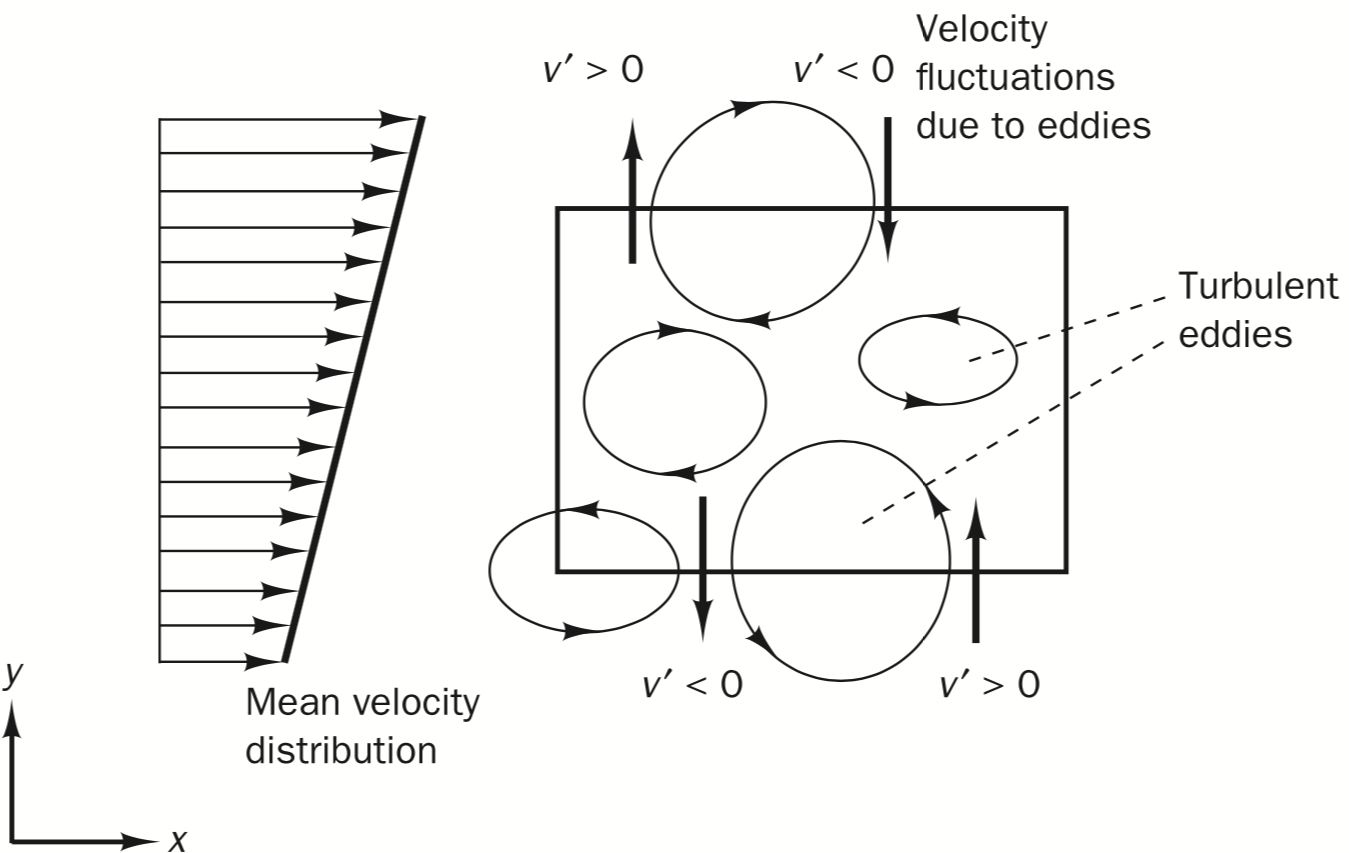
\includegraphics[width=0.5\linewidth]{fig/screenshot001}
	\label{fig:screenshot001}
\end{figure}
The net result of this mixing is momentum exchange due to convective transport by the eddies, which causes the faster moving fluid layers to be decelerated and the slower moving layers to be
accelerated. \newline 

Consequently,
the fluid layers experience additional turbulent shear stresses, which are known
as the \textbf{Reynolds stresses}.

This proves that the equations for momentum and energy are affected by these fluctuations. 

\newpage
\subsection*{RANS equations}

	By the instantaneous continuity and Navier Stokes equations we can investigate the effects of
	fluctuations on the mean flow using the Reynolds decomposition and replace the flow variables by the sum of a mean and fluctuating component. \newline 
	
	We discover that arise some terms that's involve the products of fluctuating velocities and are associated with convective momentum transfer due to turbulent eddies. 
	
	\[ \dots + \left[\dfrac{\partial(-\overline{u'w'})}{\partial x} + \dfrac{\partial(-\overline{v'w'})}{\partial y} + \dfrac{\partial(-\overline{w'^2})}{\partial z} \right]\] 
	
	This result in six additional stresses:
	\begin{itemize}
		\item Three normal stresses \[\tau_{xx} \sim \overline{u'^2} \qquad \tau_{yy} \sim \overline{v'^2} \qquad \tau_{zz} \sim \overline{w'^2}\]
		\item Three shear stresses: \[\tau_{yx} \sim \overline{u'v'} \qquad \tau_{zy} \sim \overline{v'x'} \qquad \tau_{zx} \sim \overline{w'u'}\]
	\end{itemize} 
	The extra turbulent stresses terms, are the Reynolds stresses. \newline 
	
	The
	normal stresses involve the respective variances of the x y and z velocity fluctuations they
	are always non zero because they contain squared velocity fluctuations

%\newpage
\subsection*{Turbulent flow calculations}


The
numerical methods developed to capture the important effects due to turbulence can be
grouped into the following three categories:
\begin{enumerate}
	\item \textbf{Turbulence models} for Reynolds averaged Navier Stokes (RANS) equations:
	
	The k-$\varepsilon$ model and the Reynolds stress model, which computing
	resources required for reasonably accurate flow computations are modest.
	
	\item \textbf{LES}, Large eddy simulation: 
	
	An intermediate form of turbulence calculations which tracks
	the behavior of the larger eddies. The method involves space filtering of the unsteady
	Navier Stokes equations prior to the computations, which passes the larger eddies and rejects
	the smaller eddies. 
	Large computing demand. 
	
	\item \textbf{DNS}, Direct numerical simulation:
	
	These simulations compute the mean flow and all
	turbulent velocity fluctuations. The grids comprehend the Kolmogorov scales with extra fine time steps. 	
	Very high costly method.  
\end{enumerate}

%\newpage
\section{Classical turbulence models}


In
order to be able to compute turbulent flows with the RANS equations it is necessary to
develop turbulence models to predict the Reynolds stresses and the scalar transport terms and
close the system of mean flow equations. \newline
 

The
most common RANS turbulence models are classified on the basis of the number of
additional transport equations that need to be solved along with the RANS flow equations.
\begin{figure}[H]
	\centering
	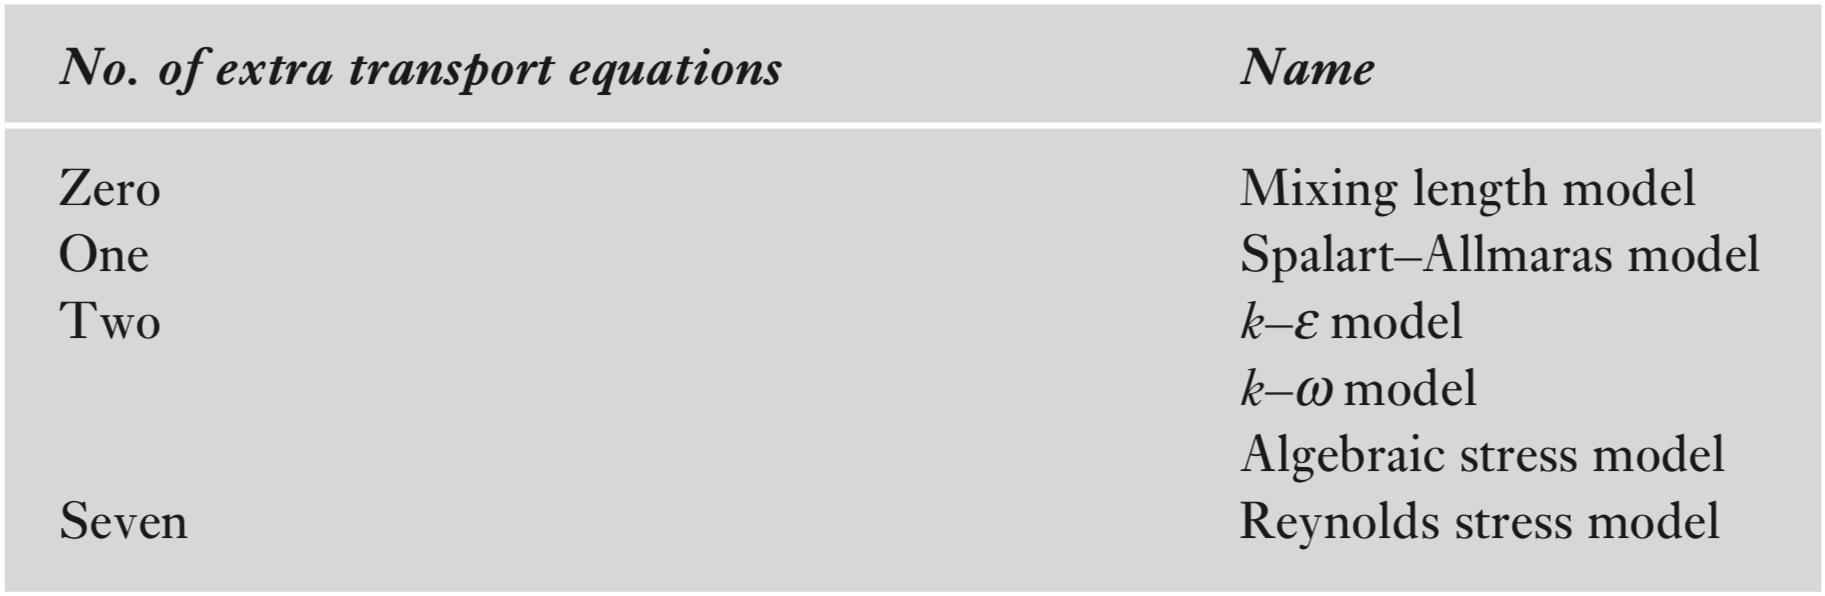
\includegraphics[width=0.5\linewidth]{fig/screenshot002}
	\label{fig:screenshot002}
\end{figure}
The mixing length and k-$\varepsilon$ models are the most widely used and
validated They are based on the presumption that there exists an analogy between the action of
viscous stresses and Reynolds stresses on the mean flow. \newline 

Both
stresses appear on the right hand side of the momentum equation, and in Newton’s law of
viscosity the viscous stresses are taken to be proportional to the rate of deformation of fluid
elements. 

Boussinesq
proposed in 1877 that Reynolds stresses might be proportional to mean rates of
deformation:
\[\tau_{ij} \sim \overline{u'_iu_j'} = \mu_t\left(\dfrac{\partial U_i}{\partial x_j} + \dfrac{\partial U_j}{\partial x_i}\right) - {2\over3}\rho k\delta_{ij}\]
where
$k$ is the turbulent kinetic energy per unit mass. \newline 


Turbulent
transport of heat, mass and other scalar properties can be modelled similarly  taken to be proportional to the gradient of the mean value of
the transported quantity`:
\[\overline{u'_i\varphi'} = \Gamma_t\dfrac{\partial \Phi}{\partial x_i}\]
where $\Gamma_t$ is the turbulent or eddy diffusivity. \newline 

Since
turbulent transport of momentum and heat or mass is due to the same mechanism  - eddy
mixing - we expect that the value of the turbulent diffusivity $\Gamma_t$ is fairly close to that of the
turbulent viscosity $\mu_t$. 

This
assumption is better known as the Reynolds analogy. 

We can now introduce a turbulent
Prandtl/Schmidt number 
\[\sigma_t = \dfrac{\mu_t}{\Gamma_t} \approx 1\]

The
\textbf{k-$\varepsilon$ model} is a more sophisticated and general, but also more costly, description of
turbulence which allows for the effects of transport of turbulence properties by convection and
diffusion and for production and destruction of turbulence.

Two
transport equations, one for the turbulent kinetic energy $k$ and one for the
rate of dissipation of turbulent kinetic energy $\varepsilon$ are solved. 

The
underlying assumption of both these models is that the turbulent viscosity $\mu_t$ is isotropic: the ratio between Reynolds stress and mean rate of deformation is the same in
all directions. 

However, this
assumption fails in many complex flows: the
six transport equations, one for each Reynolds stress, contain diffusion, pressure strain and dissipation terms whose individual effects are unknown and cannot be measured. \newline 

In
\textbf{Reynolds stress equation models} assumptions are made about these unknown terms, and the resulting
PDEs are solved in conjunction with the transport equation for the rate of dissipation of
turbulent kinetic energy $\varepsilon$. 

\newpage
\subsection{K-$\varepsilon$ model}

The
standard k-$\varepsilon$ model (1974) has two model equations, one for k and
one for $\varepsilon$ based on our best understanding of the relevant processes causing changes to these
variables. 

We
use k and $\varepsilon$ to define velocity scale $\vartheta$ and length scale $\ell$ representative of the large scale
turbulence:
\[\vartheta = k^{1\over2} \qquad \ell = \dfrac{k^{3\over2}}{\varepsilon}\]
In
words, the equations that leads are:
\begin{figure}[H]
	\centering
	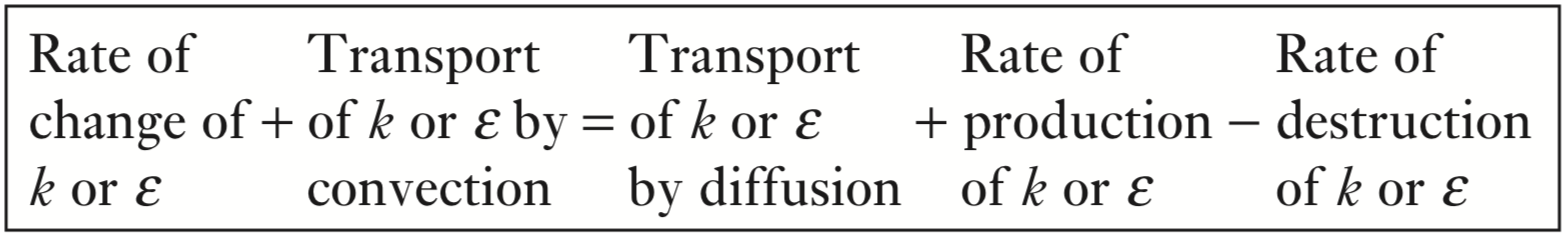
\includegraphics[width=0.5\linewidth]{fig/screenshot003}
	\label{fig:screenshot003}
\end{figure}

Production
and destruction of turbulent kinetic energy are always closely linked: dissipation rate
$\varepsilon$ is large where production of k is large. 

The
model equation for $\varepsilon$ assumes that its production and destruction terms are proportional to
the production and destruction terms of the k equation. \newline 

The
model equations for k and $\varepsilon$ are elliptic by virtue of the gradient diffusion term Their
behavior is similar to the other elliptic flow equations, which gives rise to the need for the
following boundary conditions:
\begin{itemize}
	\item Inlet;
	\item Outlet, Symmetry;
	\item Free stream;
	\item Solid Walls:
	\begin{itemize}
		\item $\uparrow~Re$ the turbulence production equals the rate of dissipation: wall functions;
		\item $\downarrow Re$ viscous effect are predominant: wall damping functions needs to be applied. 
	\end{itemize}
\end{itemize}


%\newpage
\subsection{Spalart-Allmaras model}

	The
	Spalart Allmaras model involves one transport equation for kinematic eddy viscosity
	parameter $\widetilde{\nu}$ and a specification of a length scale by means of an algebraic formula, and provides
	economical computations of boundary layers in external aerodynamics. \newline 
	
	The dynamic eddy viscosity is related to $\widetilde{v}$ by:
	\[\mu_t = \rho\widetilde{\nu}f_{\nu1}\]
	This
	equation contains the wall damping function $f_{\nu1} = f_{\nu1}\left(\frac{\widetilde{\nu}}{\nu}\right)$ which tends to unity for high
	Reynolds numbers, so the kinematic eddy viscosity parameter $\widetilde{\nu}$ is just equal to the kinematic
	eddy viscosity $\nu_t$ in this case. 
	
	At the wall the damping function $f_{\nu1}$ tends to zero. \newline 
	
	In words ew always have:
	\begin{figure}[H]
		\centering
		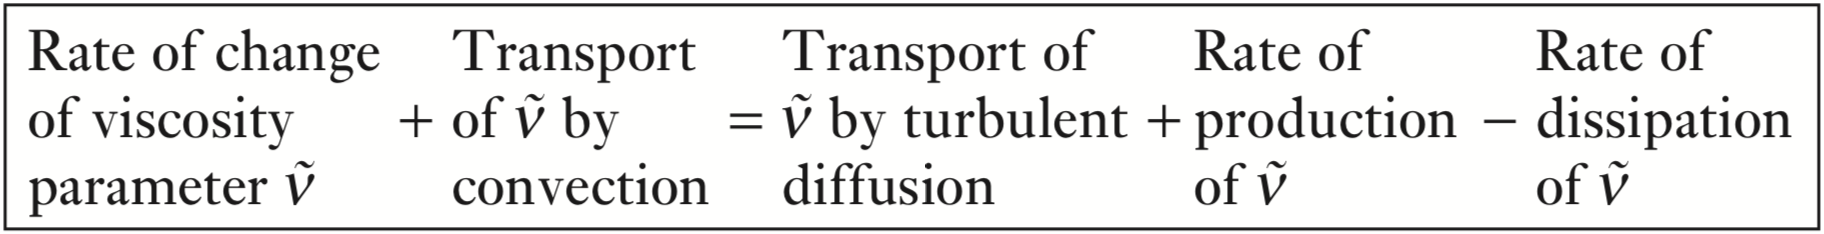
\includegraphics[width=0.5\linewidth]{fig/screenshot004}
		\label{fig:screenshot004}
	\end{figure}
	In
	the k $\varepsilon$ model the length scale is found by combining the two transported quantities k and $\varepsilon$. 
	
	In this one-equation turbulence model the length scale cannot be computed, but must be specified
	to determine the rate of dissipation of the transported turbulence quantity.
	
	So, the product $ky$ (with $y$ distance to the solid
	wall) will be used as the length scale. \newline 
	
	In
	complex geometries it is difficult to define the length scale, so the model is unsuitable for
	more general internal flows Moreover, it lacks sensitivity to transport processes in rapidly
	changing flows

%\newpage
\subsection{Wilcox k-$\omega$ model}

In
the k -$\varepsilon$ model the kinematic eddy viscosity $\nu_t$ is expressed as the product of a velocity scale $\vartheta$
and a length scale $\ell$.  

The
rate of dissipation of turbulence kinetic energy $\varepsilon$ is not the only possible length scale
determining variable: many other two equation models have been postulated. \newline 

The
most prominent alternative is the k-$\omega$ model proposed by Wilcox ('88, '93, '94 )which
uses the turbulence frequency \(\omega = \dfrac{\varepsilon}{k} \) as the second variable. 

If we use this
variable the length scale is \(\ell = \dfrac{\sqrt{k}}{\omega}\).


The eddy viscosity is given by:
\[\mu_t = \dfrac{\rho k}{\omega}\]

So, in words:
\begin{figure}[H]
	\centering
	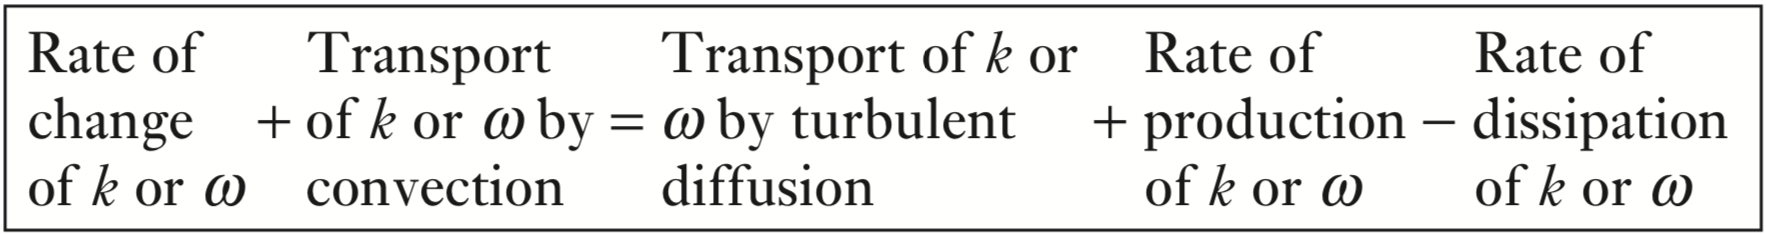
\includegraphics[width=0.5\linewidth]{fig/screenshot005}
	\label{fig:screenshot005}
\end{figure}

The
k-$\omega$ model initially attracted attention because integration to the wall does not require wall damping functions in low Reynolds number applications. 

At
inlet boundaries the values of k and $\omega$ must be specified, and at outlet boundaries the usual zero gradient conditions are used.

The
boundary condition of $\omega$ in a free stream, where turbulence kinetic energy $k\rightarrow0$ and
turbulence frequency $\omega\rightarrow0$ is the most problematic one. 

Equation
for $\mu_t$ shows that the eddy viscosity is indeterminate or infinite as $\omega\rightarrow0$ so a small
non zero value of $\omega$ must be specified. 

Unfortunately,
results of the model tend to be dependent on the assumed free stream value of
$\omega$ which is a serious problem in external aerodynamics and aerospace applications where free
stream boundary conditions are used as a matter of routine.

%\newpage
\subsection{Menter SST k-$\omega$ model}

	Menter (1992) noted that the results of the k-$\varepsilon$ model are much less sensitive to the assumed values in the free stream, but its near wall performance is unsatisfactory for boundary
	layers with adverse pressure gradients. \newline 
	
	This
	led him to suggest a hybrid model using:
	\begin{itemize}
		\item A transformation of the k-$\varepsilon$ model into a k-$\omega$
		model in the near wall region;
		\item The standard k-$\varepsilon$ model in the fully turbulent region far from the wall;
	\end{itemize}  

	The
	Reynolds stress computation and the k equation are the same as in Wilcox’s original k-$\omega$
	model, but the $\varepsilon$ equation is transformed into an $\omega$ equation by substituting $\varepsilon = k\omega$. \newline 
	
	This arise an extra source term in the model PDEs: the cross-diffusion term,
	which arises during the $\varepsilon = k\omega$ transformation of the diffusion term in the $\varepsilon$-equation. \newline 
	
	Menter (2003) summarize a series of modifications to optimize the performance of the SST
	k-$\omega$ model based on experience with the model in general purpose computation:
	\begin{itemize}
		\item \textbf{Revised model constants};
		\item \textbf{Blending
			functions}: used to achieve a smooth transition between the two models;
		\item \textbf{Limiters}: the turbulent kinetic energy production is limited to
		prevent the build up of turbulence in stagnation regions. 			
	\end{itemize}


\subsection{Turbulence models performance}

	The
	k-$\varepsilon$ model gives good results for simple flows and some recirculating flows, but research
	over a period of three decades has highlighted a number of shortcomings in low Reynolds number flows, rapidly changing flows, strong adverse pressure gradients and re-circulation
	regions. \newline 
	
	\textbf{External
	aerodynamics}: the Spalart-Allmaras, k-$\omega$ and SST k-$\omega$ models are all suitable.
	
	The SST
	k-$\omega$ model is most general, and tests suggest that it gives superior performance for zero pressure
	gradient and adverse pressure gradient boundary layers, free shear layers and a NACA 4412
	aerofoil. \newline 
	
	\textbf{General
	purpose CFD}:the k-$\omega$ and SST k-$\omega$
	models can both be applied. They both have a similar range of strengths and weaknesses as the
	k-$\varepsilon$ model and fail to include accounts of more subtle interactions between turbulent stresses
	and mean flow when compared with the RSM. 

%\newpage
\section{Large
	Eddy Simulation (LES)}

In
a turbulent flow the smaller eddies are nearly isotropic and have a universal behavior. \newline

On
the other hand, the larger eddies, which interact with and extract energy from the mean flow,
are more an-isotropic and their behavior is dictated by the geometry of the problem domain,
the boundary conditions and body forces. \newline

A
different approach to the computation of turbulent flows accepts that the larger eddies need
to be computed for each problem with a time dependent simulation. The universal behavior of
the smaller eddies, on the other hand, should hopefully be easier to capture with a compact
model. \newline

This
is the essence of the large eddy simulation approach to the numerical treatment of
turbulence. \newline 

Instead
of time averaging, LES uses a spatial filtering operation to separate the larger and smaller
eddies. 

The
method starts with the selection of a filtering function and a certain cutoff width with the
aim of resolving in an unsteady flow computation all those eddies with a length scale greater
than the cutoff width. \newline 

In
the next step the spatial filtering operation is performed on the time dependent flow
equations. During spatial filtering information relating to the smaller, filtered-out turbulent
eddies is destroyed. \newline 

The
interaction effects between the larger, resolved eddies and the smaller unresolved ones,
gives rise to sub-grid-scale stresses or SGS stresses: their effect on the resolved flow must be
described by means of an SGS model. \newline 

The
inherent unsteady nature of LES suggests that the computational requirements should be
much larger than those of classical turbulence models. 

\newpage
\section{Direct Numerical Simulation (DNS)}

	Direct
	numerical simulation of turbulent flow takes the Navier-Stokes equations set as a starting
	point and develops a transient solution on a sufficiently fine spatial mesh with sufficiently small
	time steps to resolve even the smallest turbulent eddies and the fastest fluctuations. \newline 
	
	This leads to: 
	\begin{itemize}
		\item Precise
		details of turbulence parameters;
		\item Instantaneous
		results can be generated that are not measurable with instrumentation;
		\item Advanced
		experimental techniques can be tested and evaluated. 
	\end{itemize}
	
	On the other side, is extremely computer demanding:  Moin
	and Kim (1997) estimated computing times of 100 hours to 300 years for turbulent flows at
	Reynolds numbers in the range 10$^4$ to 10$^6$ based on high performance computer speeds of 150 Mflops available at that time. 

\newpage
\part{Finite Volume Method}
\section{Diffusion problems}

	In
	this part we develop the numerical method based on the integration of transport equations
	governing fluid flow and heat transfer, the \textbf{finite volume method} by considering the simplest
	transport process of all pure diffusion in the steady state. \newline 
	
	The
	control volume integration, which forms the key step of the finite volume method that
	distinguishes it from all other CFD techniques, yields to an integrated formula of the governing equations.  

%\newpage
\subsection{1-Dimensional diffusion problems}

	Consider
	the steady state diffusion of a property $\varphi$ in a one dimensional domain defined in
	figure:
	\begin{figure}[H]
		\centering
		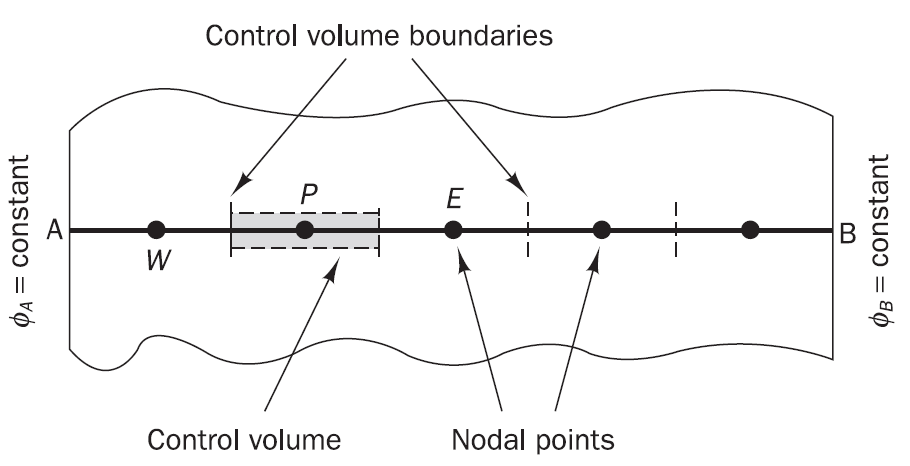
\includegraphics[width=0.5\linewidth]{fig/screenshot006}
		\label{fig:screenshot006}
	\end{figure}
	The finite volume method consists into three fundamental steps for producing a solution:
	\begin{enumerate}
		\item \textbf{Grid Generation} 
		
		We have to divide the domain into discrete control volumes. 
		
		Let us place a number of nodal points in the space between A and B. 
		
		The boundaries (or faces) of
		control volumes are positioned mid way between adjacent nodes. 
		\begin{figure}[H]
			\centering
			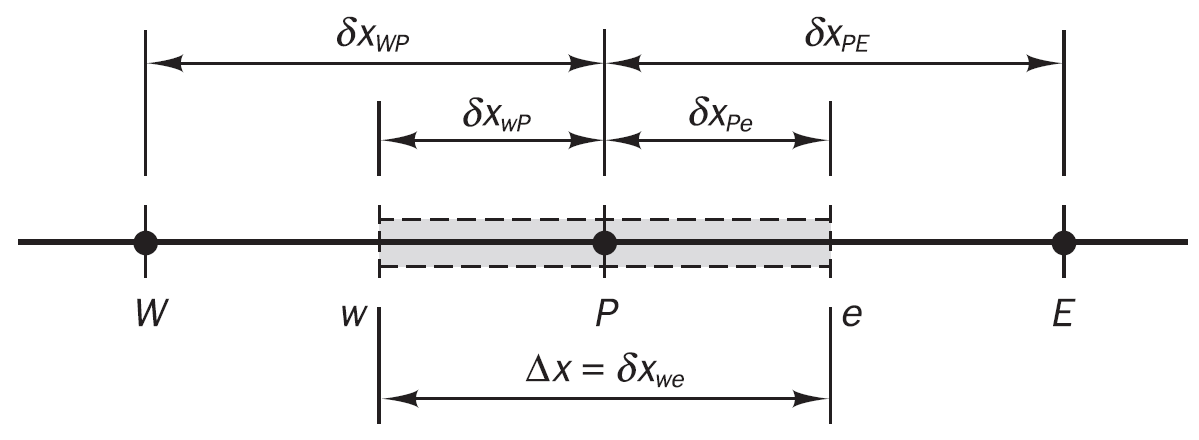
\includegraphics[width=0.5\linewidth]{fig/screenshot007}
			\label{fig:screenshot007}
		\end{figure}
		Thus,
		each node is surrounded by a control volume or cell. 
		
		It is common practice to set up
		control volumes in such a way that the physical boundaries coincide with the control volume
		boundaries. \newline 
		
		A
		general nodal point is identified by P and its neighbors in a one dimensional geometry, the
		nodes to the west and east, are identified by W and E respectively. 
		
		The
		west side face of the control volume is referred by $w$ and the east side control volume face
		by $e$.
		
		\item \textbf{Discretization} 
		
		The
		key step of the finite volume method is the integration of the governing equation over a control volume to yield a discretised equation at its nodal point P. \newline 
		
		\textbf{NB:} the discretised equation has a
		clear physical interpretation: 
		
		The diffusive flux of $\varphi$ leaving the east face minus the diffusive flux
		of $\varphi$ entering the west face is equal to the generation of $\varphi$, long story short, it constitutes a balance equation
		for $\varphi$ over the control volume. \newline 
		
		The values of the property $\varphi$ and the diffusion coefficient are
		defined and evaluated at nodal points. \newline 
		
		To
		calculate gradients (and hence fluxes) at the control volume faces an approximate distribution
		of properties between nodal points is used: the linear approximations seem to be the obvious and
		simplest way of calculating interface values and the gradients. 
		
		This
		practice is called central differencing:
		\[\Gamma_w = \dfrac{\Gamma_W+\Gamma_P}{2} \qquad \Gamma_e = \dfrac{\Gamma_P+\Gamma_E}{2}\]
		
		\item \textbf{Solution}
		
		Discretised
		equations must be set up at each of the nodal points in order to solve a problem. \newline 
		
		For
		control volumes that are adjacent to the domain boundaries the general discretised equation
		is modified to incorporate boundary conditions. \newline 
		
		The
		resulting system of linear algebraic equations is then solved to obtain the distribution of the
		property $\varphi$ at nodal points.
	\end{enumerate}

%\newpage
\subsection*{2-Dimensional diffusion problems}

	The
	methodology used in deriving discretised equations in the one dimensional case can be
	easily extended to two dimensional problems. 
	\begin{figure}[H]
		\centering
		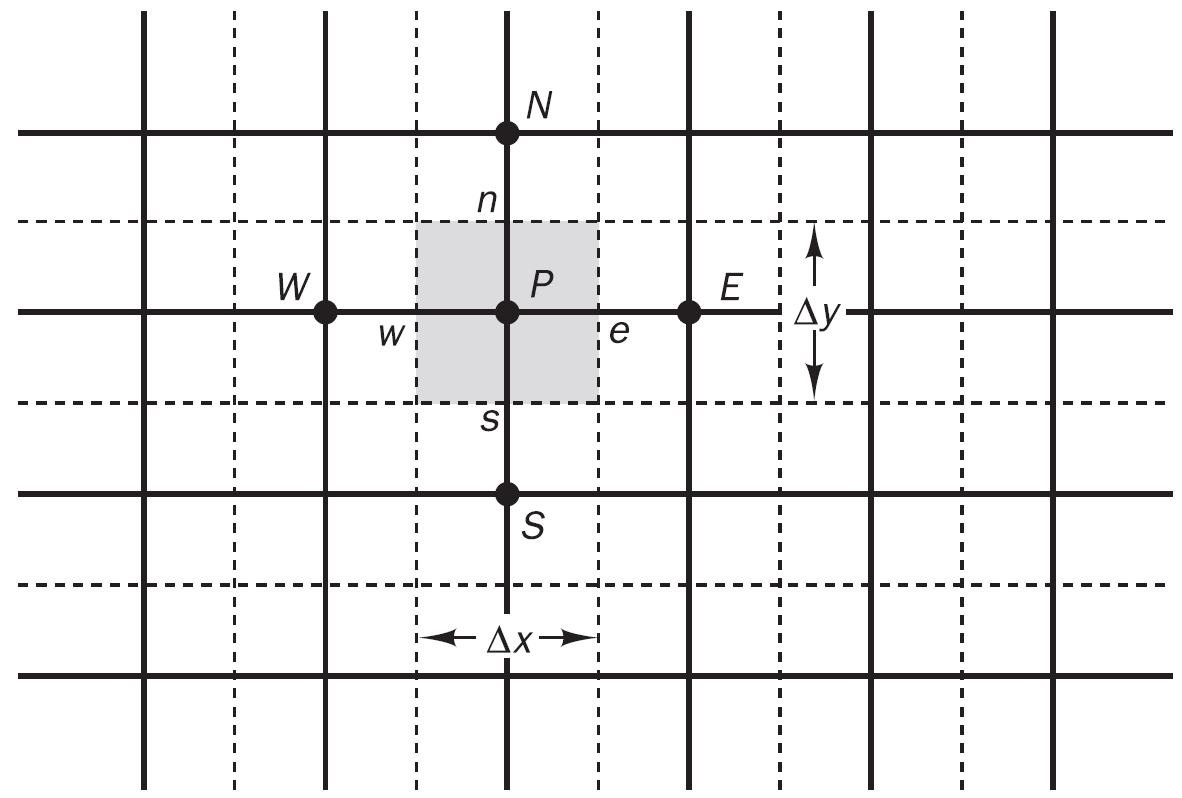
\includegraphics[width=0.4\linewidth]{fig/screenshot008}
		\label{fig:screenshot008}
	\end{figure}
	In addition to
	the east E and west W neighbours a general grid node P now also has north N and south S
	neighbours.

%\newpage
\subsection*{3-Dimensional diffusion problems}

Now
a three dimensional grid is used to sub divide the domain A typical control volume is
shown in figure
\begin{figure}[H]
	\centering
	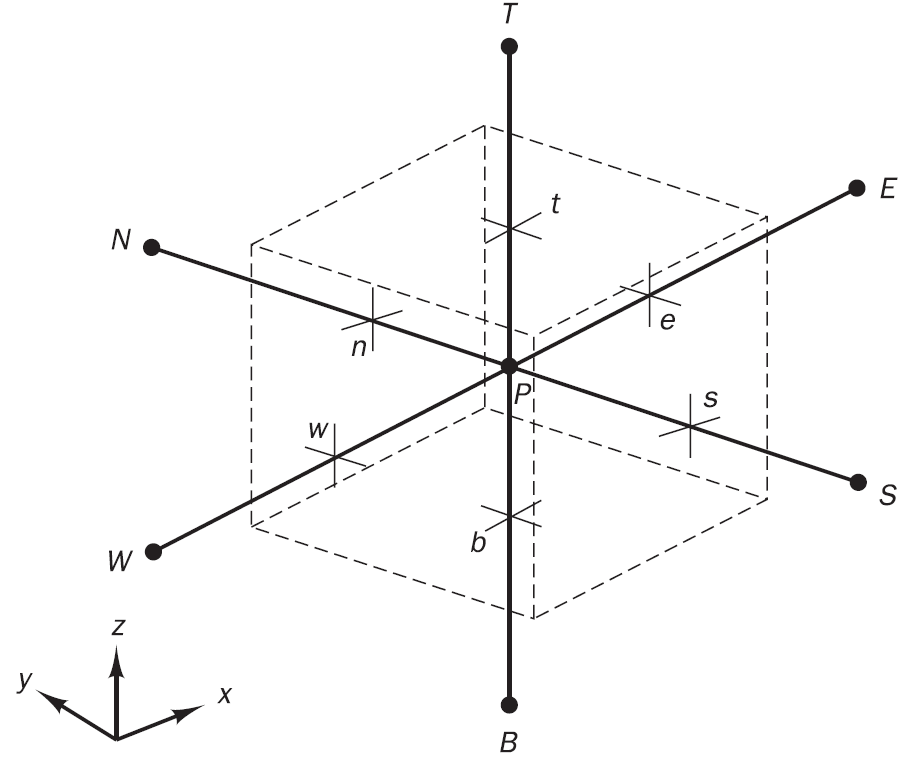
\includegraphics[width=0.4\linewidth]{fig/screenshot009}
	\label{fig:screenshot009}
\end{figure}

A
cell containing node P now has six neighbouring nodes identified as west, east, south, north,
bottom and top W, E, S, N, B, T.

As
before, the notation w e s n b and t is used to refer to the west, east, south, north, bottom
and top cell faces respectively. 

%\newpage
\section{Convection-Diffusion problems}

Diffusion
always occurs alongside convection in nature so here we examine methods to predict
combined convection and diffusion. 

The
steady convection diffusion equation can be derived from the transport equation for a
general property $\varphi$ by deleting the transient term, in integral form:
\[\int_A \textbf{n}\cdot(\rho\varphi\textbf{u})dA = \int_A\textbf{n}\cdot(\Gamma\nabla\varphi)dA + \int_{CV} S_{\varphi}dV\]
This
equation represents the flux balance in a control volume. \newline 

The LHS gives the net convective flux and the RHS contains the net diffusive
flux and the generation or destruction of the property $\varphi$ within the control volume. \newline 


\begin{tcolorbox}[colback=red!5!white,colframe=red!75!black,title=Take Home Message]
		The
	main problem in the discretisation of the convective terms is the calculation of the value of
	transported property $\varphi$ at control volume faces and its convective flux across these boundaries. 
\end{tcolorbox}

It
would seem obvious to try out the central differencing method, which worked so well for
diffusion problems also on the convective terms for obtaining discretised equations, however,
the diffusion process affects the distribution of a transported quantity along its
gradients in all directions.  

In this way the grid size become dependent on the relative strength of convection and diffusion. \newline

In a simple way, in this current analysis we assume that the velocity is "somehow" known. \newline 

Let us consider absence of source and a 1D control volume as it follows:
\begin{figure}[H]
	\centering
	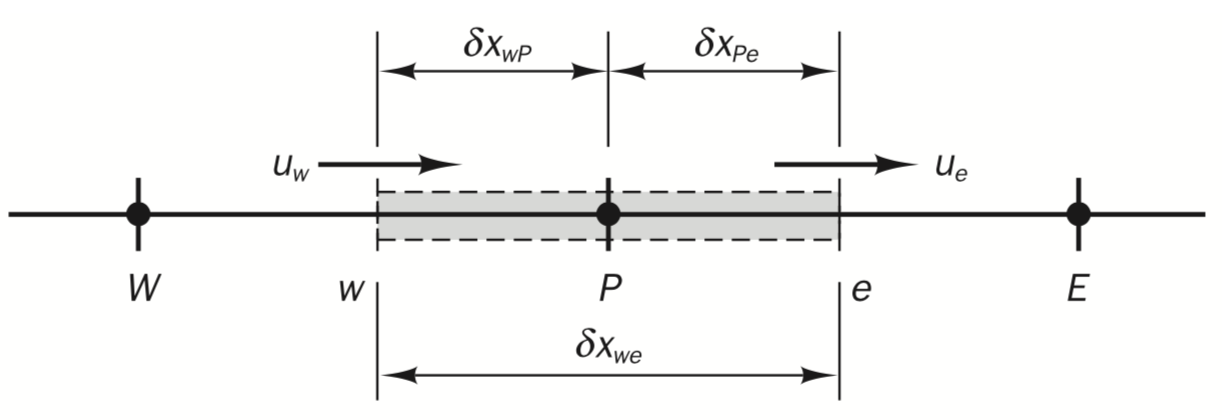
\includegraphics[width=0.5\linewidth]{fig/screenshot010}
	\label{fig:screenshot010}
\end{figure}
Our
attention is focused on a general node P. 

Steady convection and diffusion of property $\varphi$ is governed by:
\[\dfrac{d}{dx}(\rho u \varphi) = \dfrac{d}{dx}\left(\Gamma\dfrac{d\varphi}{dx}\right)\]
The
flow must also satisfy the continuity equation:
\[\dfrac{d(\rho u)}{dx} = 0\]

The Integration fo these equation leads to, respectively
\[(\rho uA\varphi)_e - (\rho uA\varphi)_w = \left(\Gamma A\dfrac{d\varphi}{dx}\right)_e - \left(\Gamma A\dfrac{d\varphi}{dx}\right)_w\]

\[(\rho uA)_e - (\rho uA)_w = 0\]

It
is convenient to define two variables $F$ and $D$ to represent the convective mass flux per unit
area and diffusion conductance at cell faces:
\[F = \rho u \qquad D = \dfrac{\Gamma}{\delta x}\]
Assuming that $A_w = A_e = A$:
\[F_e\varphi_e - F_w\varphi_w = D_e(\varphi_E-\varphi_P) - D_w(\varphi_P-\varphi_W) \]
\[F_e - F_w = 0\]

In
order to solve the convection diffusion equation we need to calculate the transported
property $\varphi$ at the $e$ and $w$ faces. \newline 

The
central differencing approximation has been used to represent the diffusion terms and it
seems logical to try linear interpolation to compute the cell face values for the convective terms
on the left hand side of the transport equation
\[\varphi_e = \dfrac{\varphi_P+\varphi_E}{2} \qquad \varphi_w = \dfrac{\varphi_W+\varphi_P}{2}\]

After some mathematical passages and after identifying
the coefficients of $\varphi_W$ and $\varphi_E$ as $a_W$ and $a_E$ the central differencing expressions for
the discretised convection diffusion equation are
\[a_P\varphi_P = a_W\varphi_W + a_E\varphi_E\]
It
can be easily recognised that the equation for steady convection diffusion problems takes the
same general form as equation for pure diffusion problems. \newline

The
difference is that the coefficients of the former contain additional terms to account for
convection. 

To
solve a one dimensional convection diffusion problem we write discretised equations for all
grid nodes. 
This
yields a set of algebraic equations that is solved to obtain the distribution of the transported
property $\varphi$.  \newline 

Otherwise,
central differencing scheme produces a solution that appears to oscillate around the exact
solution, these
oscillations are often called "wiggles" and show that often the analytical
solution is clearly not very good.  

%\newpage
\section{Discretisation scheme properties}

The
failure of central differencing scheme in certain cases involving combined convection and diffusion
forces. \newline 

in practical calculations we can only use a finite sometimes quite small number of
cells, and our numerical results will only be physically realistic when the discretisation scheme
has certain fundamental properties
\begin{enumerate}
	\item Conservativeness;
	\item Boundedness;
	\item Transportiveness. 
\end{enumerate}

%\newpage
\subsection{Conservativeness}

Integration
of the convection diffusion equation over a finite number of control volumes yields a
set of discretised conservation equations involving fluxes of the transported property $\varphi$ through
control volume faces; to
ensure conservation of $\varphi$ for the whole solution domain, the flux of $\varphi$ leaving a control volume
across a certain face must be equal to the flux of $\varphi$ entering the adjacent control volume through
the same face.


To
achieve this, the flux through a common face must be represented in a consistent manner by one and the same expression in adjacent control volumes.
\begin{figure}[H]
	\centering
	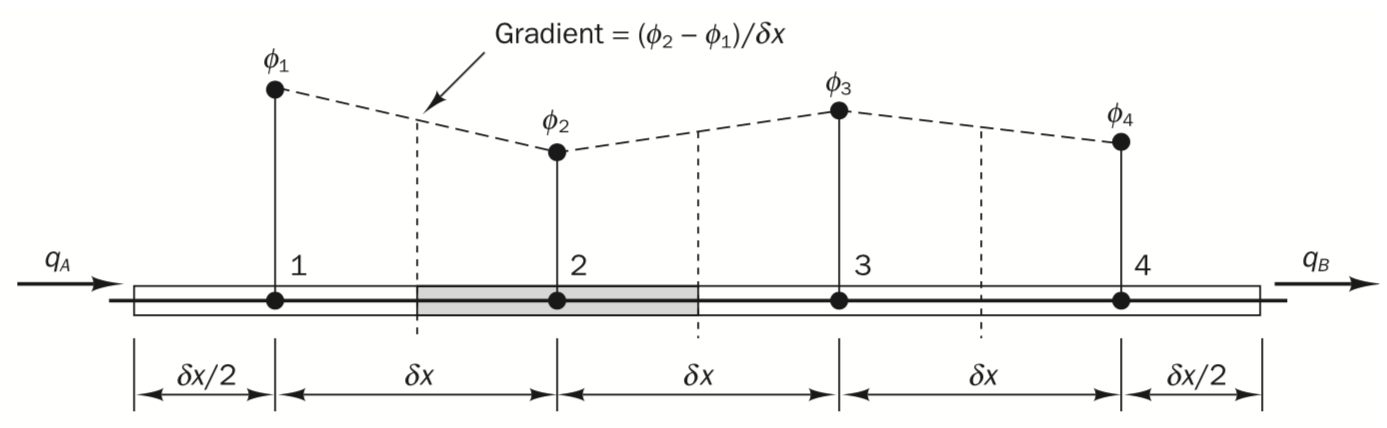
\includegraphics[width=0.5\linewidth]{fig/screenshot011}
	\label{fig:screenshot011}
\end{figure}
The
fluxes across the domain boundaries are denoted by $q_A$ and $q_B$. Let us consider four control
volumes and apply central differencing to calculate the diffusive flux across the cell faces.
\begin{figure}[H]
	\centering
	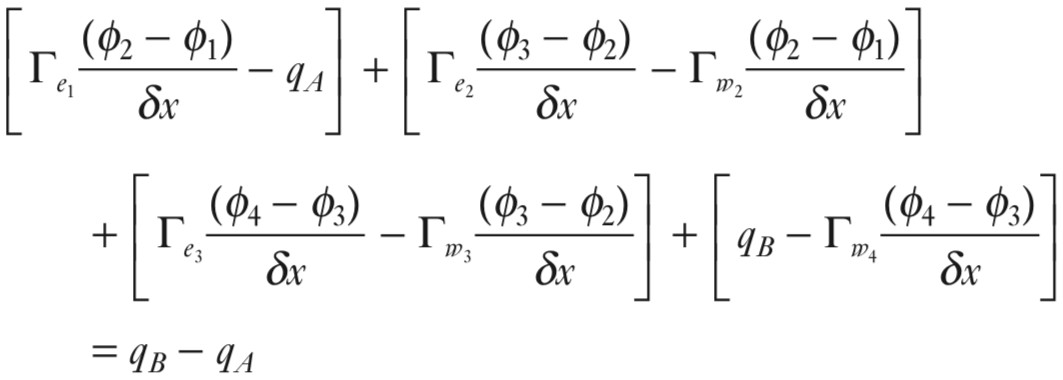
\includegraphics[width=0.5\linewidth]{fig/screenshot012}
	\label{fig:screenshot012}
\end{figure}

Since $\Gamma_{e1} = \Gamma_{w2}, \Gamma_{e2} = \Gamma_{w3}, \Gamma_{e3} = \Gamma_{w4}$ the fluxes across control volume faces are expressed in a
consistent manner and cancel out in pairs when summed over the entire domain: only
the two boundary fluxes remain in the overall balance, so the equation expresses
overall conservation of property $\varphi$. \newline 

Inconsistent
flux interpolation formulae give rise to unsuitable schemes that do not satisfy
overall conservation.

For
example, let us consider the situation where a quadratic interpolation formula:
\begin{figure}[H]
	\centering
	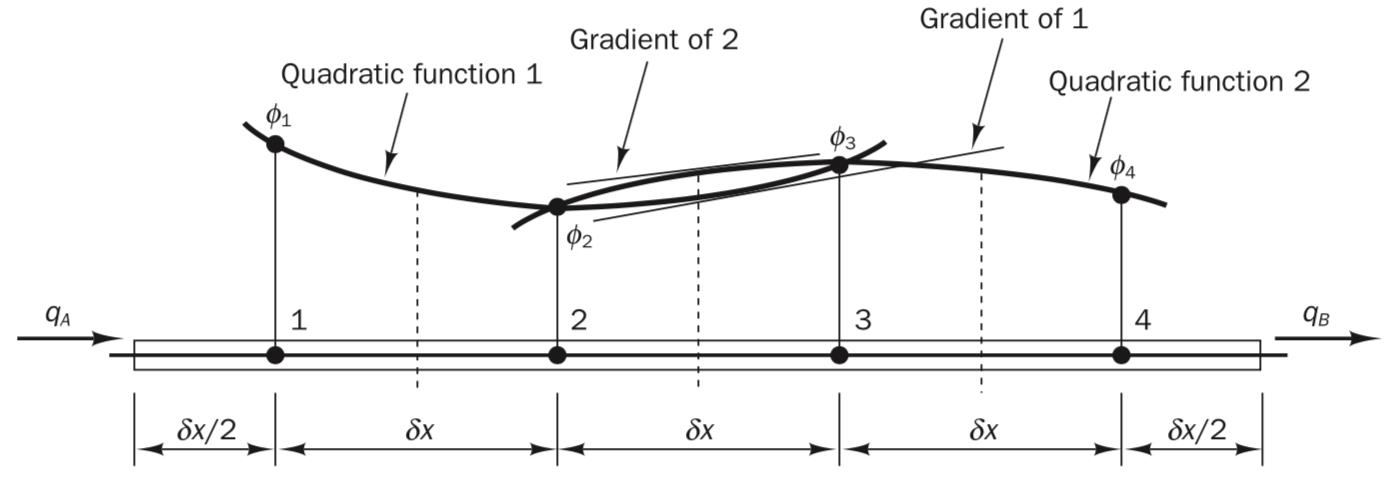
\includegraphics[width=0.5\linewidth]{fig/screenshot013}
	\label{fig:screenshot013}
\end{figure}
the flux values calculated at the east face of control volume 2 and the west face of
control volume 3 may be unequal if the gradients of the two curves are different at the cell face: this is the case when two fluxes do not cancel out when summed and overall conservation is not
satisfied. 

%\newpage
\subsection{Boundedness}

	The
	discretised equations at each nodal point represent a set of algebraic equations that needs
	to be solved. \newline 
	
	Normally
	iterative numerical techniques are used to solve large equation sets: these techniques
	start the solution process from a guessed distribution of the variable $\varphi$ and perform successive
	updates until a converged solution is obtained. \newline 
	
	Scarborough (1958) has shown that a sufficient condition for a \textbf{convergent iterative method} can be achieved if 
	the differencing scheme produces coefficients which put into a matrix, this is \textbf{diagonally dominant}. \newline 
	
	
	\begin{tcolorbox}[colback=red!5!white,colframe=red!75!black,title=Take Home Message]
		This states
	that in the absence of sources the internal nodal values of property $\varphi$ should be bounded by its
	boundary values
	\end{tcolorbox}
	
	Another
	essential requirement for boundedness is that all coefficients of the discretised
	equations should have the same sign (usually all positive). 
	
	Physically
	this implies that an increase in the variable $\varphi$ at one node should result in an increase
	in $\varphi$ at neighbouring nodes. \newline 
	
	If
	the discretisation scheme does not satisfy the boundedness requirements it is possible that the
	solution does not converge at all, or, if it does, contains "wiggles".


\subsection{Transportiveness}

The transportiveness property of a fluid flow can be illustrated by considering the
effect at a point P due to two constant sources of $\varphi$ at nearby points W and E

We define the non-dimensional cell Peclet number as a measure of the relative strengths of
convection and diffusion
\[Pe = \dfrac{F}{D}\]
The
lines in figure indicate the general shape of contours of constant $\varphi$ due to both
sources for different values of Pe.

The
value of $\varphi$ at any point can be thought of as the sum of contributions due to the two sources.

Let
us consider two extreme cases to identify the extent of the influence at node P due to the
sources at W and E
\begin{itemize}
\item No convection and pure diffusion $Pe\rightarrow0$
\item No diffusion and pure convection $Pe\rightarrow\infty$
\end{itemize}
In
the case of pure diffusion, the fluid is stagnant $Pe\rightarrow0$ and the contours of constant $\varphi$ will be
concentric circles centred around W and E since the diffusion process tends to spread $\varphi$ equally
in all directions. 

Conditions at this point are
influenced by both sources at W and E.
\begin{figure}[H]
	\centering
	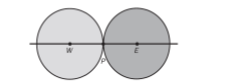
\includegraphics[width=0.5\linewidth]{fig/screenshot014}
	\label{fig:screenshot014}
\end{figure}
As Pe increases the contours change shape from circular to elliptical and are shifted in the
direction of the flow
\begin{figure}[H]
	\centering
	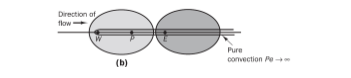
\includegraphics[width=0.5\linewidth]{fig/screenshot015}
	\label{fig:screenshot015}
\end{figure}
Influencing
becomes increasingly biased towards the upstream direction at large values of Pe.

In
the case of pure convection $Pe\rightarrow\infty$ the elliptical contours are completely stretched out in the
flow direction all of property $\varphi$ emanating from the sources at W and E is immediately
transported downstream. \newline 

Conditions at P are now unaffected by the downstream source at E and completely dictated
by the upstream source at W. \newline 

\begin{tcolorbox}[colback=red!5!white,colframe=red!75!black,title=Take Home Message]
	The
relationship between directionality of influencing (based on the flow direction) and
magnitude of the Peclet number in the discretisation scheme is known as the \textbf{transportiveness}

\end{tcolorbox}



\section{Central Differencing Scheme}

	\begin{itemize}
		\item \textbf{Conservativeness}:
		
			The central differencing scheme uses consistent expressions to evaluate
			convective and diffusive fluxes.
			
			The scheme is conservative. 
			
		\item \textbf{Boundedness}:
		\begin{enumerate}
			\item The coefficients of
			the central differencing scheme satisfy the Scarborough criterion. 
			
			\item If the convection dominates it is possible for $a_E$ to be negative, for this coefficient to be positive, must be 
			\[Pe_e<2\]
			If this condition is not respected, will be the violation of a boundedness requirements, leading to maybe not physical solutions.
		\end{enumerate}
		
		
		\item \textbf{Transportiveness}:
		
		The central differencing scheme introduces influencing at node P from the directions of
		all its neighbours to calculate the convective and diffusive flux. 
		Thus, the scheme does not recognise the direction of the flow or the strength of convection relative to
		diffusion it does not possess the transportiveness property at high Pe.
		
		\item \textbf{Accuracy}:
		
		The Taylor series truncation error of the central differencing scheme is second order. 
	\end{itemize}

%\newpage
\section{Upwinding Differencing Scheme}

The
upwind differencing scheme takes into account the flow direction
when determining the value at a cell face. 
\begin{figure}[H]
	\centering
	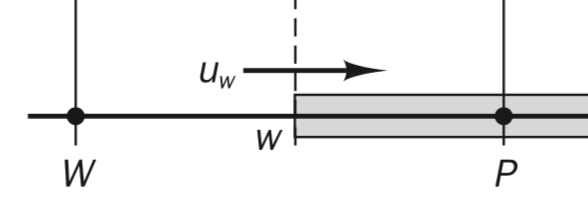
\includegraphics[width=0.3\linewidth]{fig/screenshot016}
	\label{fig:screenshot016}
\end{figure}

\begin{tcolorbox}[colback=red!5!white,colframe=red!75!black,title=Take Home Message]
	The
	convected value of $\varphi$ at a cell face is taken to be equal to the value at the upstream node.
\end{tcolorbox}
When the flow is in the positive direction:
\begin{figure}[H]
	\centering
	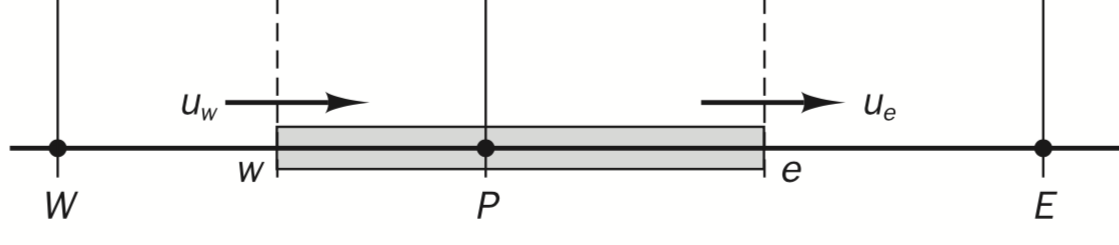
\includegraphics[width=0.5\linewidth]{fig/screenshot017}
	\label{fig:screenshot017}
\end{figure}
When the flow is in the negative direction:
\begin{figure}[H]
	\centering
	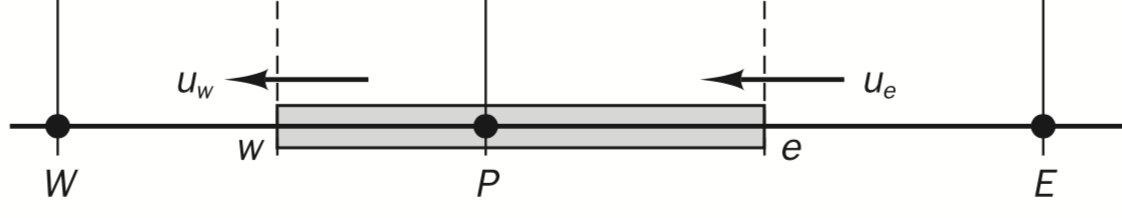
\includegraphics[width=0.5\linewidth]{fig/screenshot018}
	\label{fig:screenshot018}
\end{figure}
	\begin{itemize}
	\item \textbf{Conservativeness}:
	
	The upwind differencing scheme utilises consistent expressions to calculate
	fluxes through cell faces.
	
	\item \textbf{Boundedness}:

	The coefficients of the discretised equation are always positive and satisfy the
	requirements for boundedness. 
	
	All the coefficients are
	positive and the coefficient matrix is diagonally dominant, hence no "wiggles" occur in the
	solution.
	
	\item \textbf{Transportiveness}:
	
	The scheme accounts for the direction of the flow so transportiveness is built
	into the formulation
	
	
	\item \textbf{Accuracy}:
	
	The scheme is based on the backward differencing formula so the accuracy is only
	first order on the basis of the Taylor series truncation error
\end{itemize}

A
major \textbf{drawback} of the scheme is that it produces erroneous results when the flow is not
aligned with the grid lines: the
resulting error has a diffusion like appearance and is referred to as false diffusion.

%\newpage
\section{Hybrid Differencing Scheme}


The hybrid differencing scheme is based on a combination of central and
upwind differencing schemes.\newline

The central differencing scheme, which is second-order accurate, is employed for small Peclet
numbers and the upwind scheme, which is first-order accurate but accounts for
transportiveness, is employed for large Peclet numbers.

The hybrid differencing scheme uses piecewise formulae based on the local Peclet number to
evaluate the net flux through each control volume face. \newline 

The scheme is fully \textbf{conservative} and since the coefficients are always positive it is
unconditionally \textbf{bounded}, satisfies the \textbf{transportiveness} requirement by using an upwind formulation for large values of
Peclet number. \newline 

The \textbf{disadvantage} is that the \textbf{accuracy} in terms of Taylor series truncation error is only first-order, and makes it prone to 
diffusion errors.

%\newpage
\section{QUICK Scheme}

Formulations that do not take into account the flow direction are unstable and, therefore, more
accurate higher-order schemes, which preserve upwinding for stability and sensitivity to the flow
direction, are needed. \newline 

The quadratic upstream interpolation for convective kinetics (QUICK) scheme
uses a three-point upstream-weighted quadratic interpolation for cell face values. \newline

The face value of $\varphi$ is obtained from a quadratic function passing through two bracketing nodes
(on each side of the face) and a node on the upstream side:

\begin{figure}[H]
	\centering
	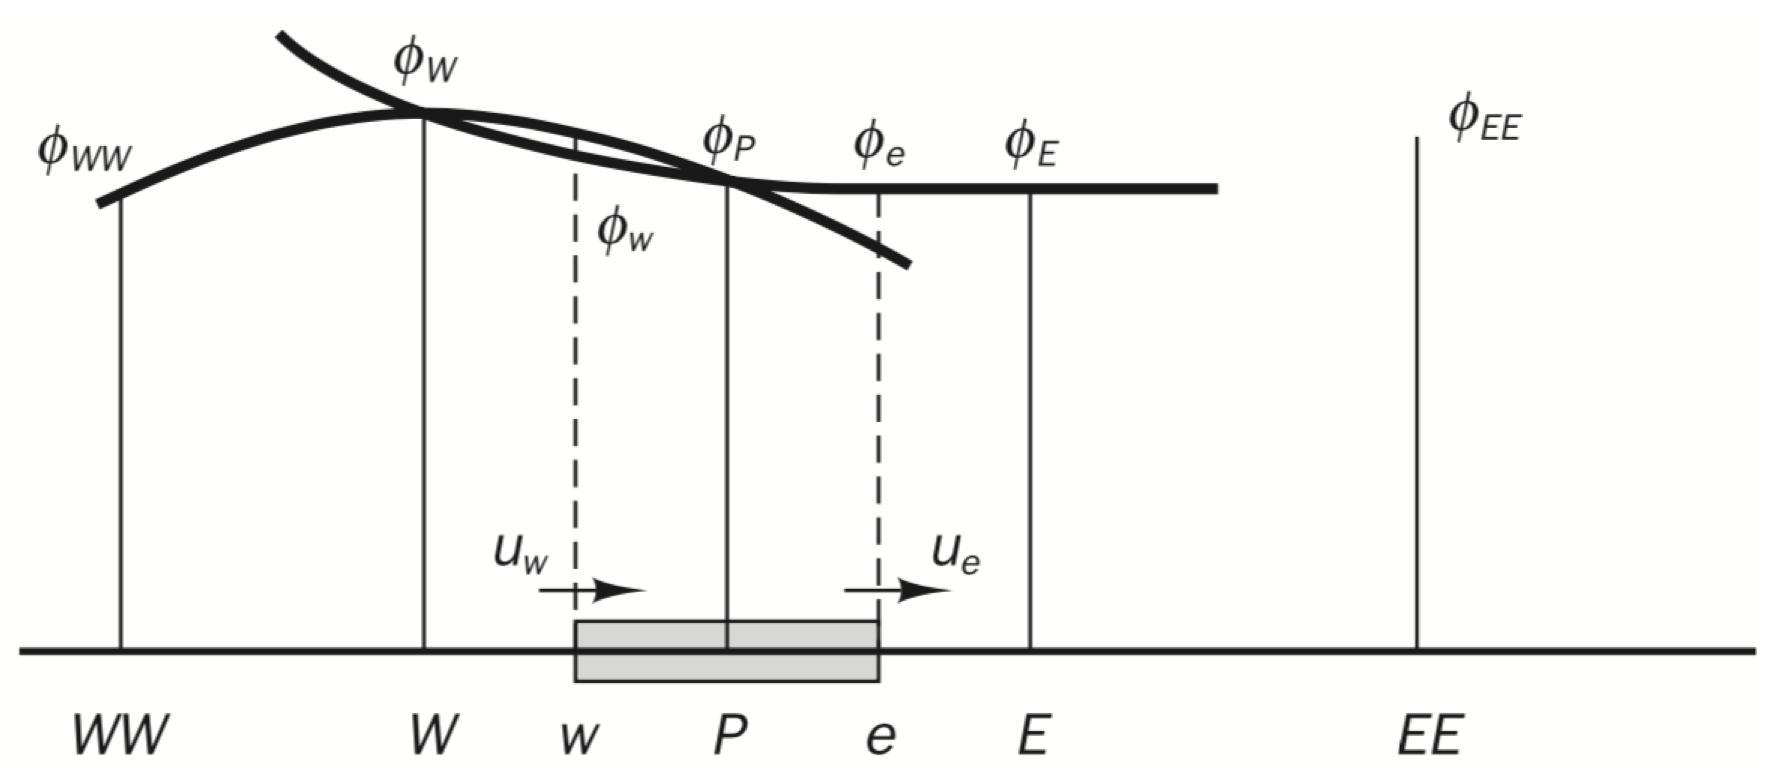
\includegraphics[width=0.5\linewidth]{fig/screenshot019}
	\label{fig:screenshot019}
\end{figure}

The diffusion terms may be evaluated using the gradient of the approximating parabola.

It is interesting to note that on a uniform grid this practice gives the same expressions as central
differencing for diffusion, since the slope of the chord between two points on a parabola is equal
to the slope of the tangent to the parabola at its midpoint. \newline 

The scheme uses consistent quadratic profiles – the cell face values of fluxes are always
calculated by quadratic interpolation between two bracketing nodes and an upstream node –
and is therefore \textbf{conservative}. \newline 

Since the scheme is based on a quadratic function its \textbf{accuracy} in terms of Taylor series
truncation error is third-order on a uniform mesh. \newline 

The \textbf{transportiveness} property is built into the scheme as the quadratic function is based on two
upstream and one downstream nodal values. If the flow field satisfies continuity the coefficient
$a_P$ equals the sum of all neighbour coefficients, which is desirable for \textbf{boundedness}.\newline

On the \textbf{downside}, the main coefficients (E and W) are not guaranteed to be positive and the
coefficients $a_{WW}$ and $a_{EE}$ are negative.

This gives rise to stability problems and unbounded solutions under certain flow conditions.

The QUICK scheme is therefore conditionally stable. \newline 

Another notable feature is the fact that the discretised equations involve not only immediate
neighbour nodes but also nodes further away. Tri-diagonal matrix solution methods are not
directly applicable. \newline 

The resultant false diffusion is small, and
solutions achieved with coarse grids are often considerably more accurate than those of the
upwind or hybrid schemes. 

\newpage
\part{Pressure - velocity coupling}
\section{Steady flows}

The
convection of a scalar variable $\varphi$ depends on the magnitude and direction of the local
velocity field.

To develop our methods in the previous parts we assumed that the velocity field
was somehow known. \newline 


In
general the velocity field is, however, not known and emerges as part of the overall solution
process along with all other flow variables. \newline 

Every
velocity component appears in each momentum equation, and the velocity field must also
satisfy the continuity equation. \newline 

The
solution of these equations is bounded with a series of intrinsic problems:
\begin{itemize}
	\item The
	convective terms of the momentum equations contain non linear quantities; 
	
	\item All
	three equations are intricately coupled: every velocity component appears in each
	momentum equation and in the continuity equation. \newline 
	
	The most complex issue to resolve is the
	role-played by the pressure: it appears in both momentum equations, but there is evidently no equation for knowing the filed of pressure.
\end{itemize}

In
general purpose flow computations we also wish to calculate the pressure field as part of the
solution, so its gradient is not normally known. \newline 


We can separate this study into two principal cases: 
\begin{enumerate}
	\item If
	the flow is \textbf{compressible} the continuity equation may be used as the transport equation for
	density and, in addition to momentum equations, the energy equation is the transport equation
	for temperature, in this way the
	pressure may be obtained from density and temperature by using the equation of state. 
	
	\item If the flow is \textbf{incompressible} the density is constant and hence by definition not linked
	to the pressure. \newline 
	
	In
	this case coupling between pressure and velocity introduces a constraint in the solution of the
	flow field and the pressure-velocity linkage can be resolved by adopting an iterative solution strategy such as the SIMPLE. 
\end{enumerate}

%\newpage
\subsection{Staggered grid}

The
finite volume method starts, as always, with the discretisation of the flow domain and of the
relevant transport equations. \newline 

First
we need to decide where to store the velocities and it seems logical to define these at the same
locations as the scalar variables such as pressure, temperature\dots

However,
if velocities and pressures are both defined at the nodes of an ordinary control volume
a highly non uniform pressure field can act like a uniform field in the discretised momentum
equations. 
\begin{figure}[H]
	\centering
	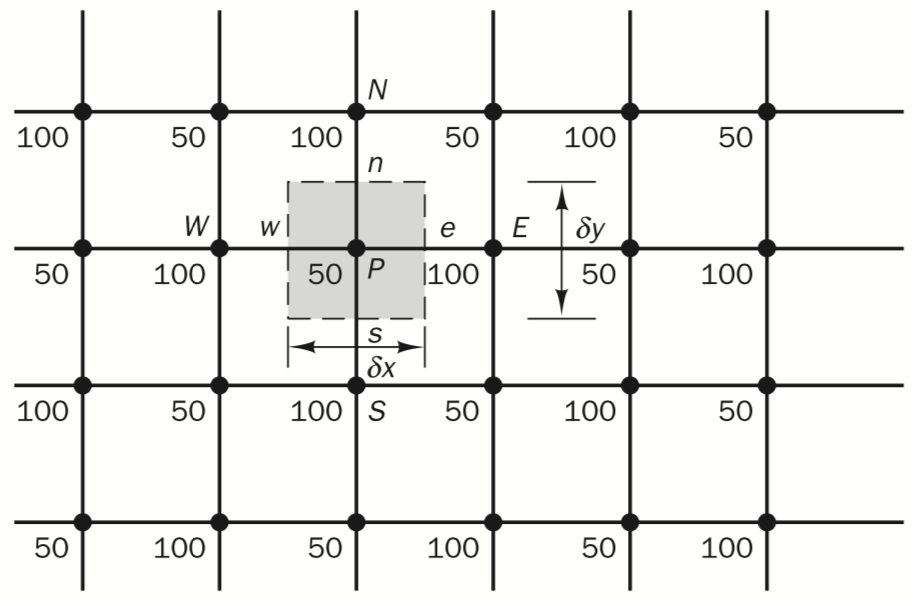
\includegraphics[width=0.5\linewidth]{fig/screenshot020}
	\label{fig:screenshot020}
\end{figure}

If
pressures at $e$ and $w$ are obtained by linear interpolation the pressure gradient terms in the $u$
and $v$ momentum equation are given by
\[\dfrac{\partial p}{\partial x} = \dfrac{p_E-p_W}{2\delta x} \qquad \dfrac{\partial p}{\partial y} = \dfrac{p_N - p_S}{2\delta y}\]
Substituting
the appropriate values from the obtained pressure field, we
find that all the discretised gradients are zero at all the nodal points even though the pressure
field exhibits spatial oscillations in both directions. 

As
a result, this pressure field would give the same (null) momentum source in the discretised
equations as a uniform pressure field: this behaviour is obviously non physical. \newline 

A
remedy for this problem is to use a \textbf{staggered grid}. \newline 


\begin{tcolorbox}[colback=red!5!white,colframe=red!75!black,title=Take Home Message]
	The
idea is to evaluate scalar variables, such as pressure, density, temperature etc at ordinary
nodal points but to calculate velocity components on staggered grid centered around the cell
faces
\end{tcolorbox}
\begin{figure}[H]
	\centering
	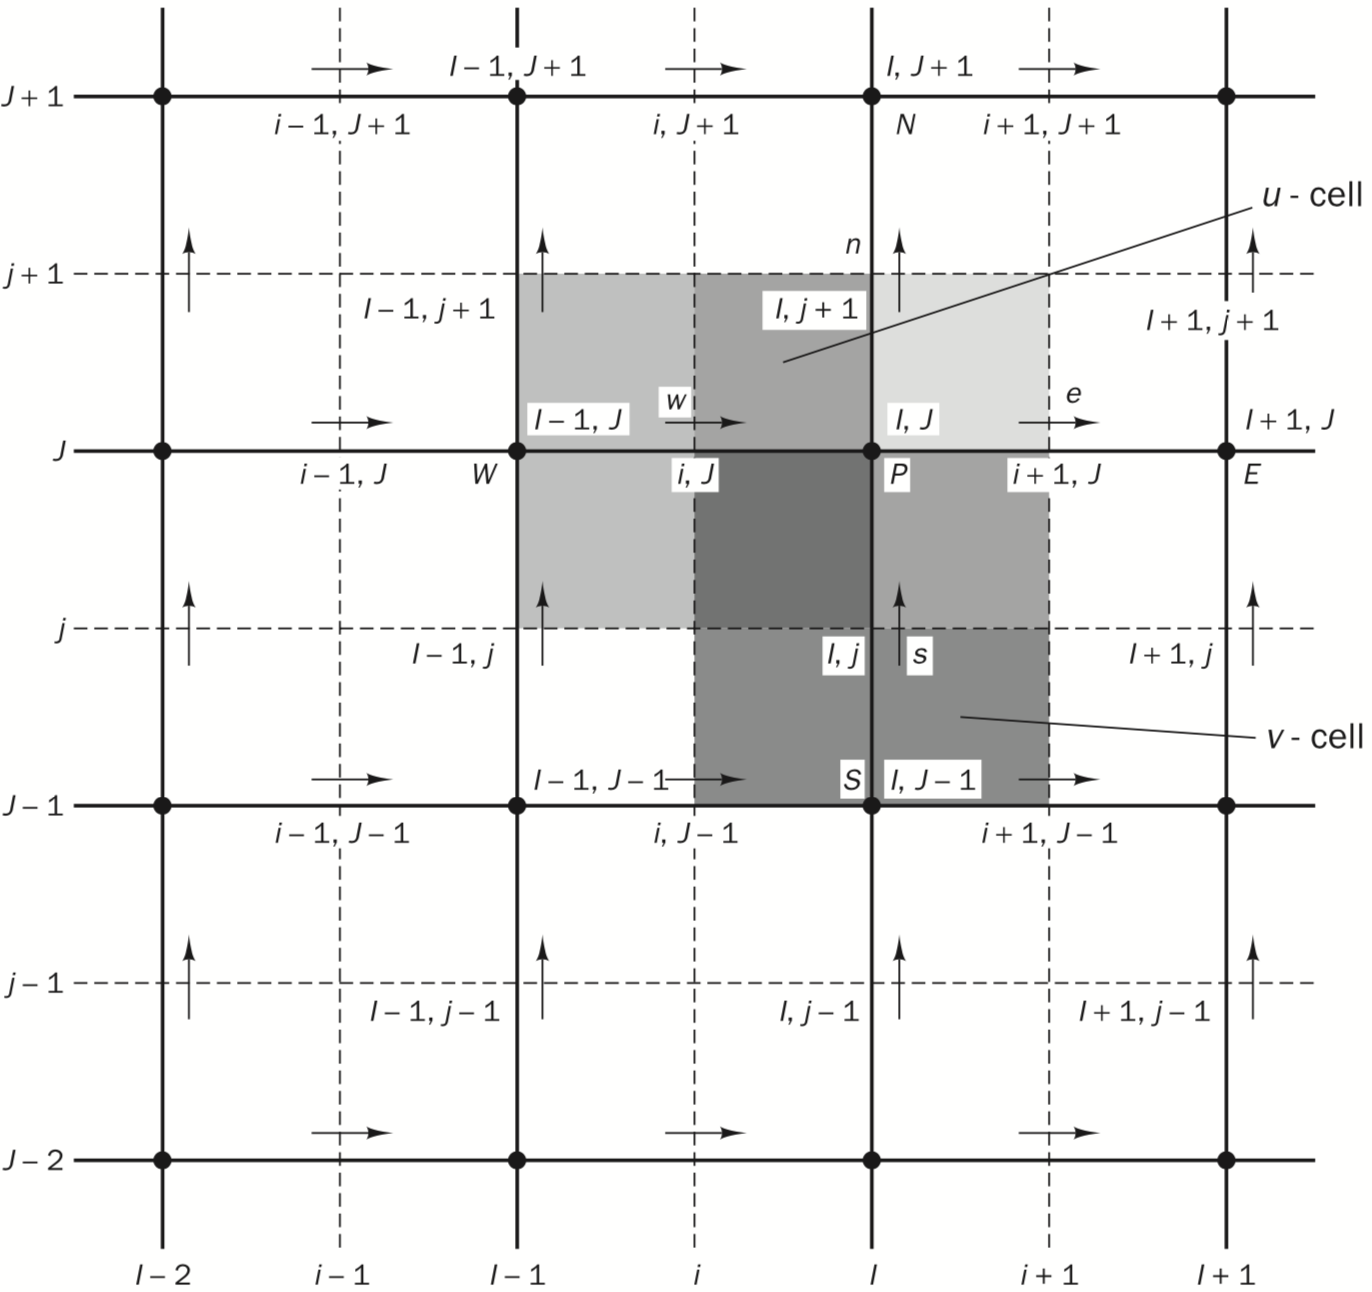
\includegraphics[width=0.5\linewidth]{fig/screenshot021}
	\label{fig:screenshot021}
\end{figure}
The
scalar variables, including pressure, are stored at the nodes marked $\bullet$ The velocities are
defined at the (scalar) cell faces in between the nodes and are indicated by arrows: horizontal $\rightarrow$
arrows indicate the locations for $u$ velocities and vertical $\uparrow$ ones denote those for $v$
velocity. \newline 

In
the staggered grid arrangement, the pressure nodes coincide with the cell faces of the $u$ and
$v$ control volumes. 

The pressure gradient terms are given by

\[\dfrac{\partial p}{\partial x} = \dfrac{p_P-p_W}{\delta x_u} \qquad \dfrac{\partial p}{\partial y} = \dfrac{p_P - p_S}{2\delta y_v}\]

If
we consider the "chessboard" pressure field again, substitution of the appropriate nodal
pressure values into these equations now yields very significant non zero pressure gradient
terms. \newline 

The
staggering of the velocity avoids the unrealistic behaviour of the discretised momentum
equation for spatially oscillating pressures. \newline 


A
further \textbf{advantage} of the staggered grid arrangement is that it generates velocities at exactly
the locations where they are required for the scalar convection diffusion transport
computations, hence,
no interpolation is needed to calculate velocities at the scalar cell faces.\newline 

Always remembering that the values of single coefficients may be calculated with any of the differencing methods
(hybrid, QUICK\dots) suitable for convection diffusion problems. \newline 

\textbf{If
	the pressure field is correct the resulting velocity field will satisfy continuity. As the pressure
	field is unknown, we need a method for calculating pressure}


%\newpage
\section{SIMPLE algorithm}

The
acronym SIMPLE stands for Semi Implicit Method for Pressure Linked Equations and is
essentially a guess and correct procedure for the calculation of pressure on the staggered grid
arrangement. \newline 

To
initiate the SIMPLE calculation process a pressure field $p^*$ is guessed. 

Discretised momentum
equations are solved using the guessed pressure field to yield velocity components $u^*$ and $v^*$, at this point
we define the correction $p'$ as the difference between correct pressure field $p$ and the
guessed pressure field $p^*$ so that
\[p = p^* + p'\]
Similarly
we define velocity corrections $u'$ and $u'$ to relate the correct velocities $u$ and $v$ to the
guessed velocities $u^*$ and $v^*$. \newline 

The
pressure correction equation is susceptible to divergence unless some under relaxation is
used during the iterative process:
\[p^{new} = p^* + \alpha_pp'\]
Taking
$\alpha_p$ between 0 and 1 allows us to add to guessed field $p^*$ a fraction of the correction field
$p'$ that is large enough to move the iterative improvement process forward, but small enough to
ensure stable computations. Also the
velocities are under relaxed. \newline 

A
correct choice of under relaxation factors $\alpha$ is essential for cost effective simulations, too
large value may lead to oscillatory or even divergent iterative solutions, and too small values will cause extremely slow convergence. 

Unfortunately,
the optimum values of under relaxation factors are flow dependent and must be
sought on a case by case basis. \newline 

The
SIMPLE algorithm gives a method of calculating
pressure and velocities. 

The
method is iterative, and when other scalars are
coupled to the momentum equations the calculation
needs to be done sequentially.

%\newpage
\section{SIMPLER algorithm}

The
SIMPLER (SIMPLE Revised) algorithm is an improved version of SIMPLE. \newline 

In
this algorithm the discretised continuity equation is used to derive a discretised equation for
pressure, instead of a pressure correction equation as in SIMPLE. 

Thus
the intermediate pressure field is obtained directly without the use of a correction. 

Velocities
are, however, still obtained through the velocity corrections of SIMPLE, in this way, not using a guessed pressure, we obtain a sort of pseudo-velocities.   \newline 


From
the discretised momentum equations, the
velocity components $u^*$ and $v*$ are obtained. \newline 

The
velocity correction equations of the SIMPLE
algorithm are used in the SIMPLER algorithm to
obtain corrected velocities. 

Therefore,
the $p'$-equation must also be solved to
obtain the pressure corrections needed for the
velocity corrections. 

%\newpage
\section{SIMPLEC algorithm}

The SIMPLEC (SIMPLE-Consistent) algorithm follows the same
steps as the SIMPLE algorithm. \newline 

The difference is that the momentum equations are manipulated so that the SIMPLEC velocity
correction equations omit terms that are less significant than those in SIMPLE. \newline 

The discretised pressure correction equation is the same as in SIMPLE, except that the d-terms
are calculated as above. \newline 

The sequence of operations of SIMPLEC is identical to that of SIMPLE.


\section{PISO algorithm}

The
PISO algorithm, which stands for Pressure Implicit with Splitting of Operators,
is a pressure-velocity calculation procedure developed originally for non iterative computation
of unsteady compressible flows. \newline 

PISO
involves \textbf{one} predictor step and \textbf{two} corrector steps and it can be seen as an extension of
SIMPLE, with a further corrector step to enhance it.

\paragraph*{Predictor Step} \mbox{} \\
Discretised
momentum equations are solved with a guessed or intermediate pressure field $p^*$ to
give velocity components $u*$ and $v^*$ using the same method as the SIMPLE algorithm. 

\paragraph*{Corrector Step 1} \mbox{} \\
The $u*$ and $v^*$ fields will not satisfy continuity unless the pressure field $p^*$ is correct. \newline 

The first corrector step of SIMPLE is introduced to give a velocity field $(u^{**}, v^{**})$ which satisfies
the discretised continuity equation. \newline 

The resulting equations are the same as the velocity correction equations of SIMPLE but, since
there is a further correction step in the PISO algorithm, we use a slightly different notation:

\[p^{**} = p^* + p' \qquad u^{**} = u^* + u' \qquad v^{**} = v^* + v'\]

As
in the SIMPLE algorithm, these equations are substituted into the discretised continuity
equation to yield pressure correction equation.

In
the context of the PISO method, this pressure correction equation is called the \textit{first} pressure
correction equation and it's solved to yield the first pressure correction field $p'$. 

Once these the pressure corrections are
known, the velocity components $u^{**}$ and $v^{**}$ can be obtained.

\paragraph*{Corrector Step 2} \mbox{} \\
To
enhance the SIMPLE procedure PISO performs a second corrector step. \newline 

A
twice corrected velocity field $(u^{***}, v^{***})$ may be obtained by solving the momentum
equations once more, using in this step the $u^{**}$ and $v^{**}$ velocities calculated in the
previous step. \newline 

Substitution of $u^{***}$ and $v^{***}$ in the discretised continuity equation yields a second pressure
correction equation, by solving this equation, a second pressure correction field $p"$ is
obtained, and the twice-corrected pressure field is calculated from:

\[p^{***} = \underbrace{p^{**}}_{= p^* + p'} + p" = p^* + p' + p"\]

The
PISO algorithm solves the pressure correction equation
twice so the method requires additional storage for
calculating the source term of the second pressure
correction equation. \newline 

Although
this method implies a considerable increase in
computational effort it has been found to be efficient and
fast. 

%\newpage
\section{Final remarks}


\begin{itemize}
	\item The
	\textbf{SIMPLE} algorithm is relatively straightforward and has been successfully implemented in
	numerous CFD procedures. \newline 
	
	the pressure correction $p'$ is satisfactory for correcting velocities but not so good for
	correcting pressure. 
	
	\item The improved procedure \textbf{SIMPLER} uses the pressure corrections to
	obtain velocity corrections only.  \newline 
	
	A
	separate, more effective, pressure equation is solved to yield the correct pressure field, by the way, no terms are omitted to derive the discretised pressure equation in SIMPLER, the obtained
	correct pressure field results in the correct velocity field. \newline 
	
	Consequently,
	the method is highly effective in calculating the pressure field correctly. 
	
	\item \textbf{SIMPLEC}
	and \textbf{PISO} have proved to be as efficient as SIMPLER in certain types of flows, but it is
	not clear whether it can be categorically stated that they are better than SIMPLER. 
\end{itemize}

Comparisons
have shown that the performance of each algorithm depends on the flow
conditions, the degree of coupling between the momentum equation and scalar equations, the amount of under relaxation used, and sometimes even on the details of the
numerical technique used for solving the algebraic equations. 

\newpage
\part{Solution of discretised equations}

In
the previous parts we have discussed methods of discretising the governing equations of fluid flow and heat transfer. \newline 

This
process results in a system of linear algebraic equations which needs to be solved.\newline 

The
complexity and size of the set of equations depends on:
\begin{itemize}
	\item The
	dimensionality of the problem;
	\item The
	number of grid nodes;
	\item The
	discretisation practice
\end{itemize}

There
are two families of solution techniques for linear algebraic equations
\begin{enumerate}
	\item \textbf{Direct methods}: Cramer’s rule matrix inversion and Gaussian elimination
	
	\item \textbf{Iterative methods}: Jacobi and Gauss Seidel point iterative methods
\end{enumerate}

The
total number of operations cannot be predicted in advance, and it is not possible to
guarantee convergence unless the system of equations satisfies some defined criteria. \newline 

\begin{itemize}
	\item The
	\textbf{TDMA} is a direct method for 1 D situations, but it can be applied iteratively to solve multi
	dimensional problems. 
	
	TDMA
	is computationally inexpensive and has the advantage that it requires a minimum amount
	of storage. 
	
	\item The
	\textbf{Jacobi} and \textbf{Gauss Seidel} methods are general purpose point iterative algorithms that are
	easily implementable, but their convergence rate can be slow when the system of equations is
	large. 
	
	\item More recently \textbf{multigrid} acceleration techniques have improved the convergence rates
	of iterative solvers to such an extent that they are now the method of choice in commercial CFD
	codes. 
\end{itemize}



%\newpage
\section{Thomas algorithm (TDMA)}


Consider a system of equations that has a tri-diagonal form, the general form of \textbf{any}
single equation is:
\[-\beta_j\phi_{j-1} + D_J\phi_j-\alpha_j\phi_{j+1} = C_j\]
And it can be rewritten as 
\[\phi_j = \dfrac{\alpha_j}{D_J}\phi_{j+1}  + \dfrac{\beta_j}{D_j}\phi_{j-1} + \dfrac{C_j}{D_j} \]

These
equations can be solved by \textbf{forward elimination} and \textbf{back substitution}. \newpage 

This process starts by eliminating of the $\phi_{j-1}$ value in the $\phi_{j+1}$ formula by substituting this value with the $\phi_j$ formula previously obtained. 
\begin{figure}[H]
	\centering
	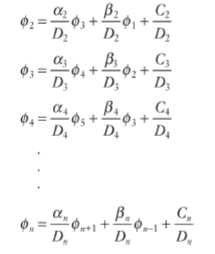
\includegraphics[width=0.3\linewidth]{fig/screenshot022}
	\label{fig:screenshot022}
\end{figure}

In the above derivation of the TDMA we assumed that boundary values $\phi_1$ and $\phi_{n+1}$ were given.

%\newpage
\subsection*{Thomas algorithm 2D}

The
TDMA can be applied iteratively to solve a system of equations for two dimensional
problems.
\begin{figure}[H]
	\centering
	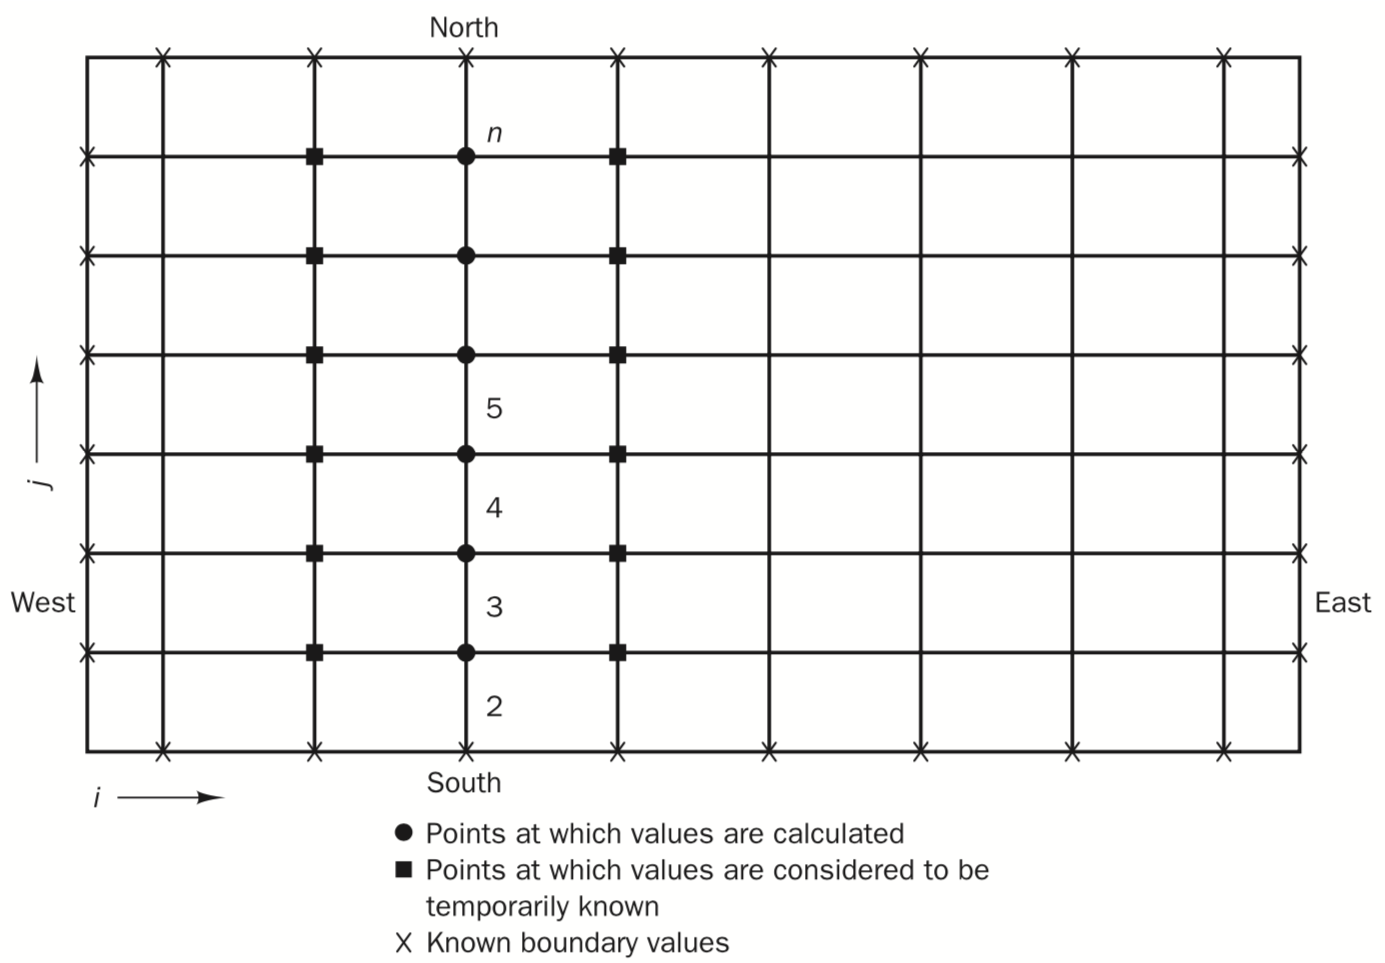
\includegraphics[width=0.5\linewidth]{fig/screenshot023}
	\label{fig:screenshot023}
\end{figure}

To
solve the system, the TDMA is applied along chosen path, e. g. north south (n-s) lines. 

Subsequently
the calculation is moved to the next north south line. \newline 

The
sequence in which lines are moved is known as the \textbf{sweep direction}.

If
we sweep from west to east the values of $\phi_W$ to the west of a point P are known from the
calculations made on the previous line. 

Values
of $\phi_E$ to its east, however, are unknown so the solution process must be iterative. 

At
each iteration cycle $\phi_E$ is taken to have its value at the end of the previous iteration or a given initial/guessed value at the first iteration. \newline 

The
line by line calculation procedure is repeated several times until a converged solution is
obtained. 


\newpage
\subsection*{Thomas algorithm 3D}

For
three dimensional problems the TDMA is applied line by line on a selected plane and then
the calculation is moved to the next plane, scanning the domain plane by plane.

\begin{figure}[H]
	\centering
	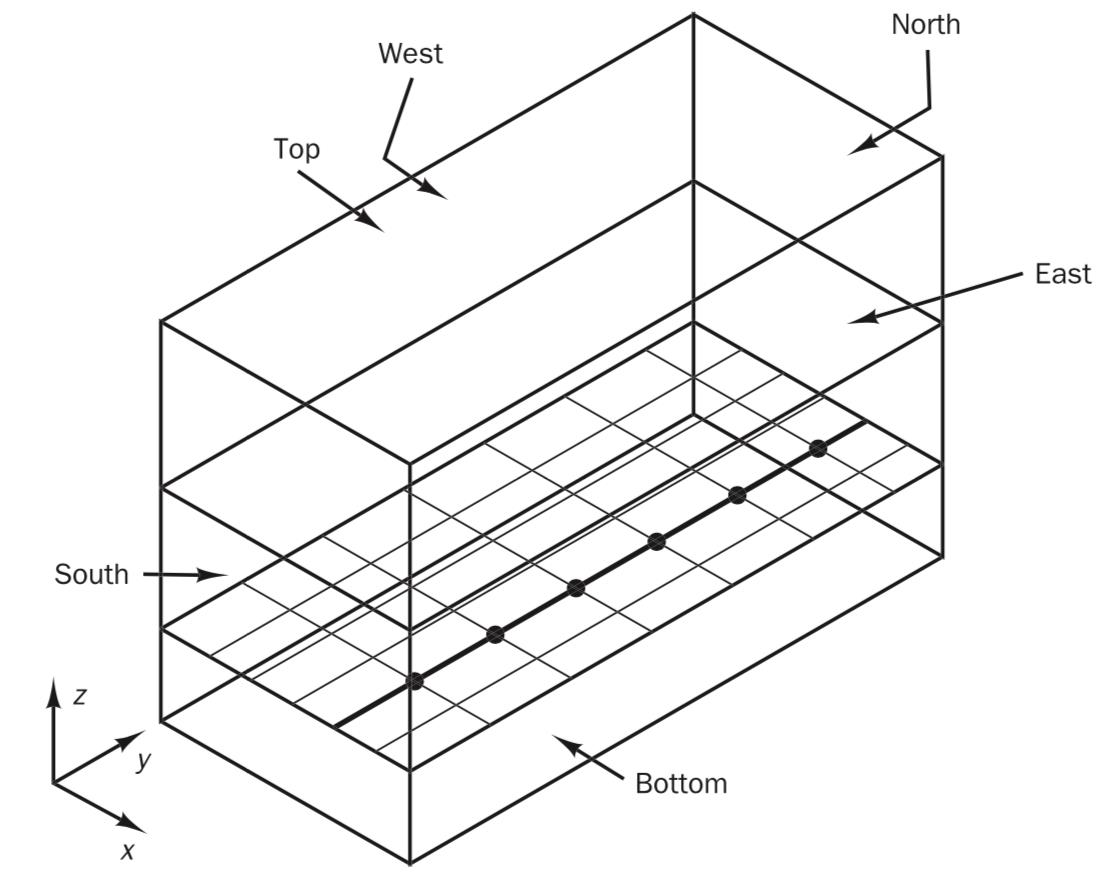
\includegraphics[width=0.5\linewidth]{fig/screenshot024}
	\label{fig:screenshot024}
\end{figure}

In
two and three dimensional computations the convergence can often be accelerated by
alternating the sweep direction so that all boundary information is fed into the calculation more
effectively, sweeping from
upstream to downstream along the flow direction produces faster convergence than sweeping
against the flow or parallel to the flow direction. \newline 


The TDMA algorithm may cause problems in unsteady flow calculations because can only be applied by incorporating several neighbouring contributions in the
source term. \newline 

A
generalised version of the TDMA, known as the penta diagonal matrix algorithm, is available
Basically
a sequence of operations is carried out on the original matrix to reduce it to upper
triangular form, and subsequently the back substitution is performed to obtain the solution. 

%\newpage
\section{Point-iterative methods}

Point
iterative techniques consists to isolate the unknown value in the respective equation en substitute the remaining unknowns with some guessed initial values.

After obtaining the first solution, this is substitute in place of the last guessed initial values. 

This
process is repeated until there is no more change in the solution. \newline 

One
condition for the iteration process to be convergent is that the matrix must be diagonally
dominant
When
general systems of equations are solved it is sometimes necessary to rearrange the
equations, but the finite volume method yields diagonally dominant systems as part of the
discretisation process, so this aspect does not require special attention. 

\subsection{Jacobi Method}
In
the Jacobi method, the unknown values at the $k$ iteration $(x_1^k\dots n_n^k)$ in the LHS are evaluated by substituting in the RHS the last known values at the previous iteration $k-1$. \newline 

To generalize, a $n\times n$ system of equation can be written as
\[\sum_{j=1}^{n}a_{ij}x_j = b_i\]

The single equation who leds a solution can be written as 
\[a_{ii}x_i = b_i - \sum_{j=1}^{n}a_{ij}{x_j}\]

By introducing the iterations, the Jacobi method consists in:
\[x_i^k = \sum_{j=1}^{n}\left(\dfrac{-a_{ij}}{a_{ii}}\right){x_j^{k-1}} + \dfrac{b_i}{a_{ii}}\]

In matrix form:
\[X^k = T\cdot X^{k-1} + C\]
Where the iteration matrix is
\[T=T_{ij} = \begin{dcases}
	\begin{aligned}
		- \dfrac{a_{ij}}{a_ii} &\qquad \text{if}~i\ne j \\
	0 &\qquad \text{if}~i= j 
	\end{aligned}
\end{dcases}\]

\subsection{Gauss - Seidel Method}

In
the Jacobi method the right hand side is evaluated using the results of the previous iteration level or from the initial guess. 

If
all the right hand sides could be evaluated simultaneously there would be no further
discussion, \textbf{but in most computing machines the calculations are performed sequentially}. \newline 


\begin{tcolorbox}[colback=red!5!white,colframe=red!75!black,title=Take Home Message]
	The
	Gauss Seidel method proceeds by making direct use of the recently available solution value and calculates by this, the next. 
\end{tcolorbox}

\[x_i^k =\sum_{j=1}^{n}\left(\dfrac{-a_{ij}}{a_{ii}}\right){x_j^{k}} \underbrace{+\sum_{j=1}^{n}\left(\dfrac{-a_{ij}}{a_{ii}}\right){x_j^{k-1}} + \dfrac{b_i}{a_{ii}}}_{\text{solution obtained by the previous iteration}}\]


The
convergence rate of the Jacobi and Gauss Seidel methods depends on the properties of the
iteration matrix.
It
has been found that these can be improved by the introduction of a so called relaxation
parameter $\alpha$. 

When
we choose $0<\alpha<1$ the procedure is an under relaxation method, whereas $\alpha>1$ is called
over relaxation. 

The
introduction of the relaxation parameter $\alpha$ changes the iteration path without changing the
final solution. \newline 

We
define the residual $r_i^k$ of the $i^{th}$ equation after $k$ iterations as the difference:
\[r_i^k = b_i - \sum_{j=1}^na_{ij}x_j^k\]
As
the iteration process is convergent the intermediate solution vector $x_j^k$ should get
progressively closer to final solution vector $x_j^{k\rightarrow\infty}$, at the same time, the $r_i^k \underset{k\rightarrow\infty}{\rightarrow} 0$. 

The
relaxation may be advantageous if we select an optimum value of $\alpha$ that minimises the
number of iterations required to reach the converged solution. 

Unfortunately,
the optimum value of the relaxation parameter is problem and mesh dependent,
and it is difficult to give precise guidance. 



\subsection{Multigrid methods} 
The
convergence rate of iterative methods such as the Jacobi and Gauss Seidel, rapidly reduces
as the mesh is refined. \newline 

The
concept of residual already introduced can be used to obtain a measure of the closeness to
the true solution of an intermediate solution in an iteration sequence. \newline 

The
average residual  $\bar{r}$ over all $n$ equations in the system is a useful indicator of iterative
convergence for a given problem
\[\bar{r} = \dfrac{1}{n}\sum_{i=1}^{n}|r_i|\]
If
the iteration process is convergent the average residual $\bar{r}\rightarrow0$. \newline 

The
average residual for a given solution parameter, is usually
normalised to make it easier to interpret its value from case to case and to compare it with
residuals relating to other solution parameters. 

The
most common normalisation is to consider the ratio of the average residual after $k$ iterations
and its value at the first iteration
\[R_{norm}^k = \dfrac{\bar{r}^k}{\bar{r}^1}\]

As
we said, within the CFD code it is possible to improve the
convergence rate by adjusting solution parameters, including
relaxation parameters, but for the sake of consistency all solution
parameters were kept constant in this case. \newline 

The
pattern of residual reduction is evident from the diagram
After a rapid initial reduction of the residuals their rate of decrease
settles to a more modest final value

\begin{figure}[H]
	\centering
	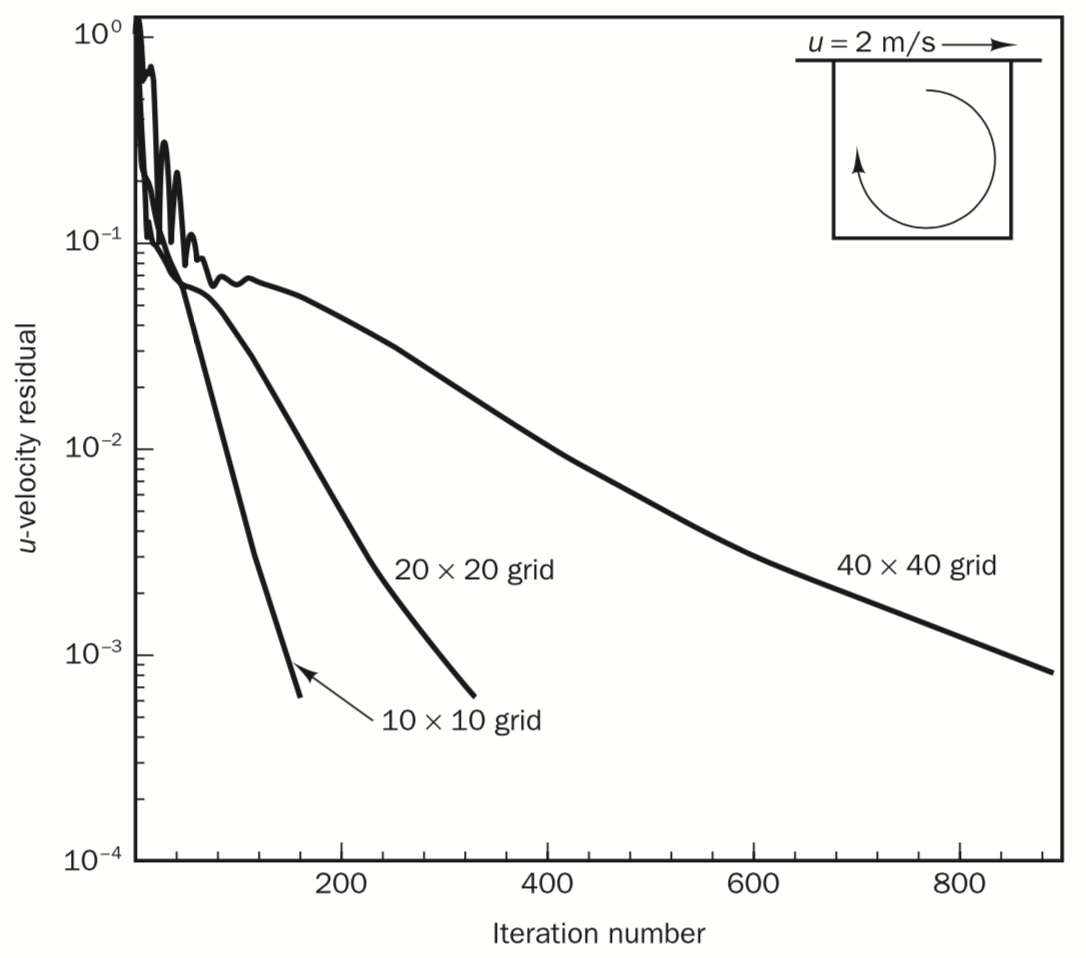
\includegraphics[width=0.5\linewidth]{fig/screenshot025}
	\label{fig:screenshot025}
\end{figure}

It
is also clear that the final convergence rate is lowest for the
finest mesh. 
If
we tried an even finer mesh, it would take even longer to
converge. \newline 

It
has been established that the solution error has components with a range of wavelengths that
are multiples of the mesh size. Iteration
methods cause rapid reduction of error components with short wavelengths up to a few
multiples of the mesh size. 

However,
long wavelength components of the error tend to decay very slowly as the iteration
count increases. \newline 

In figure can be seen that for
the coarse mesh, the longest possible wavelengths of error components (those of the
order of the domain size) are just within the short wavelength range of the mesh and all
error components reduce rapidly. On
the finer meshes, however, the longest error wavelengths are progressively further outside
the short wavelength range for which decay is rapid. \newline 

Multigrid
methods are designed to exploit these inherent differences of the error behaviour and
use iterations on meshes of different size. \newline 

The
short wavelength errors are effectively reduced on the finest meshes, whereas the long
wavelength errors decrease rapidly on the coarsest meshes. 
Moreover,
the computational cost of iterations is larger on finer meshes than on coarse meshes,
so the extra cost due to iterations on the coarse meshes is offset by the benefit of much
improved convergence rate.

\paragraph*{Multigrid procedure} 
\begin{enumerate}
	\item \textbf{Fine grid iterations} 
	
	Perform
	iterations on the finest grid with mesh spacing $h$ to generate an intermediate solution $Y^h$. \newline 
	
	The
	number of iterations is chosen sufficiently large that the short wavelength oscillatory
	component of the error is effectively reduced, but no attempt is made to eliminate the long
	wavelength error component. \newline 
	
	The
	residual vector $R^h$ for the solution on this mesh satisfies 
	\[R^h = B-A^h\cdot Y^h\]
	And the error vector $E^h$
	is given by 
	\[E^h = X-Y^h\]
	We
	have also established that the error and residual are related as follows 
	\[A^h\cdot E^h = R^h\]
	
	
	\item \textbf{Restriction}
	
	The
	solution is transferred from the fine mesh with spacing $h$ onto a coarse mesh with spacing
	$ch$ where $c>1$. 
	
	Due
	to the larger mesh spacing of the coarse mesh the long wavelength error (on the fine mesh)
	appears as a short wavelength error on the new mesh and will reduce rapidly. 
	
	
	\item \textbf{Prolongation}
	
	After
	obtaining the converged solution of error vector $E^{ch}$ for the coarse mesh we need to
	transfer it back to the fine mesh but note that we have fewer data than points in the fine mesh. \newline 
	
	We
	use a convenient interpolation operator to generate values for the
	prolonged error vector $E^{'h}$ at intermediate points in the fine mesh. 
	
	\item \textbf{Correction \& final iterations}
	
	Once
	we have calculated the prolonged error vector $E^{'h}$ we may correct the intermediate fine
	grid solution
	\[Y^{impro} = Y^h+E^{'h}\]
	Because
	the long wavelength error has been eliminated, this improved solution is closer to the
	true solution vector. \newline 
	
	However,
	several approximations were made, so we perform a few more iterations with the
	improved solution to iron out any errors that may have been introduced during restriction and
	prolongation. 
\end{enumerate}

\part{Finite volume method - Unsteady flows}
The
conservation law for the transport of a scalar in an unsteady flow has the general form:
\[\dfrac{\partial}{\partial t}(\rho\phi) + \nabla\cdot(\rho \textbf{u}\phi) = \nabla\cdot(\Gamma\nabla\phi) + S_\phi\]
The
first term of the equation represents the rate of change term and is zero for steady flows to
predict transient problems we must retain this term in the discretisation process.

The
finite volume integration of this equation over a control volume must be augmented
with a further integration over a finite time step $\Delta t$. \newline 

The
control volume integration is essentially the same as in steady flows and the same measures
are again adopted to ensure successful treatment of convection, diffusion and source terms
Here
we focus our attention on methods necessary for the time integration. 

\paragraph*{1-Dimension flows} \mbox{} \\
\[\rho c\dfrac{\partial T}{\partial t} = \dfrac{\partial}{\partial x}\left(k\dfrac{\partial T}{\partial x}\right) + S\]
\begin{figure}[H]
	\centering
	\label{fig:screenshot026}
	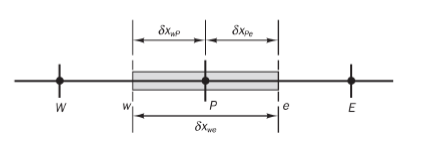
\includegraphics[width=0.5\linewidth]{fig/screenshot026}
\end{figure}
If
the temperature at a node is assumed to prevail over the whole control volume, the LHS can be written as - using a first order (backward) differencing
scheme:
\[\int\limits_{CV} \left[\int\limits_{t}^{t+\Delta t}\rho c\dfrac{\partial T}{\partial t}\right]dV = \rho c(T_P-T_P^0)\Delta V\]
Applying central differencing scheme to the RHS
\[\int\limits_{t}^{t+\Delta t}\left[\left(k_eA\dfrac{T_E-T_P}{\delta x_{PE}}\right)- \left(k_wA\dfrac{T_P-T_W}{\delta x_{WP}}\right)\right]dt + \int\limits\limits_{t}^{t+\Delta t}\bar{S}dVdt\]

To
evaluate the right hand side of this equation we need to make an assumption about the
variation of $T_P T_E$ and $T_W$ with time. 

We may generalise the approach by means of a weighting parameter $\vartheta$ between 0 and 1 and
write the integral $I_T$ of temperature $T_P$ with respect to time as:
\[I_T = \int\limits_{t}^{t+\Delta t}T_Pdt = [\vartheta T_P + (1+\vartheta)T_P^0]\Delta t\]
We
have highlighted the following values of integral $I_T$ 
\begin{itemize}
	\item If $\vartheta =0$ the temperature at old time level $t$ is used and the resulting scheme is called \textbf{explicit};
	\item If $0<\vartheta \leq 1$ temperatures at the new time level are used on both sides of the equation and
	the resulting schemes are called \textbf{implicit};
	\item If $\vartheta = 1$ the temperature at new time level $t + \Delta t$ is used and the scheme if \textbf{fully implicit};
	\item If $\vartheta = {1\over2}$ the temperatures at $t$ and $t + \Delta t$ are equally weighted and the scheme is called \textbf{Crank-Nicolson} scheme.
\end{itemize} 
So the
exact form of the final discretised equation depends on the value of $\vartheta$
\begin{figure}[H]
	\centering
	\label{fig:screenshot027}
	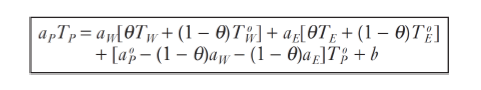
\includegraphics[width=0.5\linewidth]{fig/screenshot027}
\end{figure}

The substitution of  $\vartheta =0$ gives the \textbf{explicit} discretisation of the unsteady conductive heat
transfer equation:
\begin{figure}[H]
	\centering
	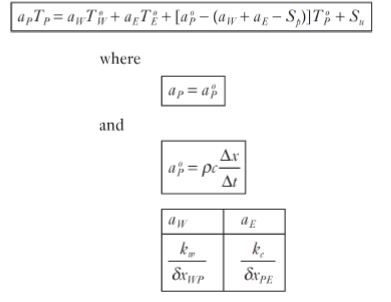
\includegraphics[width=0.5\linewidth]{fig/screenshot028}
	\label{fig:screenshot028}
\end{figure}

For
boundedness requirements, all coefficients need to be positive in the discretised equation.

For
the coefficient of $T_P^0$ to be positive we must have $a_P^0-a_w-a_e>0$, which for
constant k and uniform grid spacing ($\delta x = \Delta x$) can be written as
\[\Delta t < \rho c\dfrac{\Delta x^2}{2k}\]
This
inequality sets a stringent maximum limit to the time step size and represents a serious limitation for
the explicit scheme
It becomes very expensive to improve spatial accuracy because the maximum possible time step needs to
be reduced as the square of $\Delta x$ Consequently, this method is not recommended for general transient problems. \newline 


Using instead the \textbf{Crank Nicolson} scheme leads to:
\[\Delta t < \rho c\dfrac{\Delta x^2}{k}\]
This
time step limitation is only slightly less restrictive than that of the explicit method. 

The
Crank Nicolson method is based on central differencing and hence it is second order accurate in
time. \newline 

With \textbf{fully implicit} scheme both
sides of the equation contain temperatures at the new time step, and a system of algebraic
equations must be solved at each time level. 

It
can be seen that all coefficients are positive, which makes the implicit scheme unconditionally
stable for any size of time step.

Since
the accuracy of the scheme is only first order in time, small time steps are needed to
ensure the accuracy of results.

The
implicit method is recommended for general purpose transient calculations because of its
robustness and unconditional stability. \newline 

\textbf{The extension to unsteady 2D and 3D diffusion problems is made by quoting the fully implicit
	method due to its superior stability.}
	
\section{Transient SIMPLE}

Algorithms such as SIMPLE, for the calculation of steady flows, may be extended to transient
calculations.

The discretised momentum equations will now include transient terms formulated with the
procedure described until now.
An additional term is also required in the pressure correction equation. \newline 

The
pressure correction equation is derived from the continuity equation and should therefore
contain terms representing its transient behaviour. \newline 

In
transient flow calculations with the implicit formulation, the iterative procedures described for
steady state calculations employing SIMPLE, SIMPLER or SIMPLEC are applied at each time level
until convergence is achieved. 

\section{Transient PISO}

The
PISO algorithm is a non iterative calculation procedure in its transient version all time
dependent terms are retained in the momentum and continuity equations: the basic equations and steps involved in the transient version of the PISO algorithm
are the same as those for steady state version. \newline 

Its shows that the temporal accuracy achieved by the predictor corrector process for
pressure and momentum is third order $(\Delta t^3)$ and fourth order $(\Delta t^4)$ respectively. \newline 

Therefore,
the pressure and velocity fields obtained at the end of the PISO process with a
suitably small time step are considered to be accurate enough to proceed to the next time step immediately.

Since
the algorithm relies on the higher order temporal accuracy gained by the splitting
technique, small time steps are recommended to ensure accurate results. \newline

Since
the PISO method does not require iterations within a time level it is less expensive than the
implicit SIMPLE algorithm. 


\part{Boundary conditions}
All
CFD problems are defined in terms of initial and boundary conditions It is important that the user
specifies these correctly and understands their role in the numerical algorithm. 

In
transient problems the initial values of all the flow variables need to be specified at all solution points
in the flow domain. \newline 

The most commons boundary conditions are: 
\begin{itemize}
	\item Inlet;
	\item Outlet;
	\item Wall;
	\item Prescribed pressure;
	\item Symmetry.
\end{itemize}
In
constructing a staggered grid arrangement, we set up additional nodes surrounding the
physical boundary:
\begin{figure}[H]
	\centering
	\label{fig:screenshot029}
	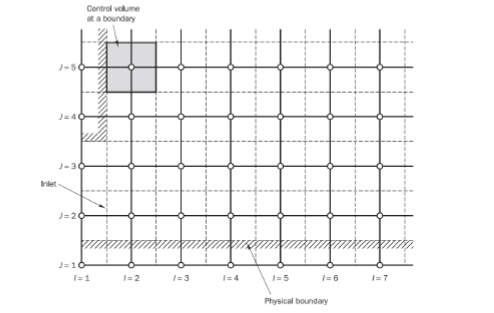
\includegraphics[width=0.5\linewidth]{fig/screenshot029}
\end{figure}
The
calculations are performed at internal nodes only. \newline

Two
notable features of the arrangement are 
\begin{enumerate}
	\item The physical boundaries coincide with scalar
	control volume boundaries;
	
	\item The nodes just outside the inlet of the domain are available to store the inlet conditions.
\end{enumerate}

We
make the following assumptions (i) the flow is always subsonic,(ii) k-$\varepsilon$ turbulence
modelling is used (iii) the hybrid differencing method is used for discretisation and (iv) the
SIMPLE solution algorithm is applied. 

\subsection*{Inlet}

The
distribution of all flow variables needs to be specified at inlet boundaries. 

As
mentioned, the grid extends outside the physical boundary and the nodes along the line are used to store the inlet values of flow variables; just
downstream of this extra node we start to solve the discretised equation for the first internal
cell. \newline 

Since
the velocity is known at inlet, it is also not necessary to make a velocity correction here. 

\paragraph{Reference pressure} \mbox{} \\
The
pressure field obtained by solving the pressure correction equation does not give absolute
pressures, so its common practice to fix the absolute pressure at one inlet node and set the pressure
correction to zero at that node, once having specified a reference value, the absolute pressure field inside the domain can now be
obtained. 

\paragraph{Estimation of k \& $\varepsilon$} \mbox{} \\
The
most accurate simulations can only be achieved by supplying measured inlet values of
turbulent kinetic energy k and dissipation rate $\varepsilon$
However,
such data are often not available in this case commercial CFD codes often estimate k
and $\varepsilon$ with approximate formulae based on a turbulence intensity.

\subsection*{Outlet}
If
the location of the outlet is selected far away from geometrical disturbances the flow
eventually reaches a fully developed state where no change occurs in the flow direction.

In
such a region we can place an outlet surface and state that the gradients of all variables
(except pressure) are zero in the flow direction.

It
is normally possible to make a reasonably accurate prediction of the flow direction far away
from obstacles. \newline 

Figures
show grid arrangements near such an outlet boundary.
The
last cells upstream of the outlet, for which a discretised equation is solved, have been
shaded and, as before, active neighbours and faces have been highlighted. \newline

This
gives us the opportunity to locate the outlet surface perpendicular to the flow direction and
take gradients in the direction normal to the outlet surface equal to zero. 

\begin{figure}[H]
	\centering
	\label{fig:screenshot033}
	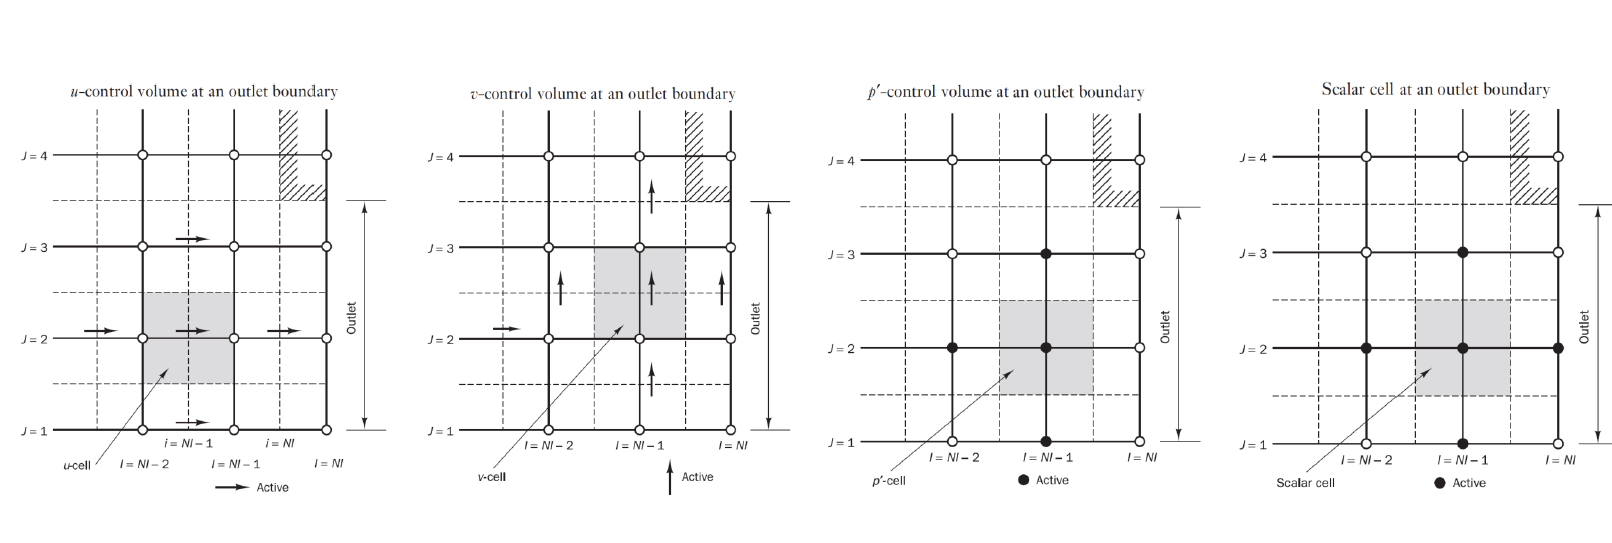
\includegraphics[width=0.7\linewidth]{fig/screenshot033}
\end{figure}

If
NI is the total number of nodes in the $x$ direction, equations are solved for cells up to I (or i) = 
NI-1

Before
the relevant equations are solved the values of flow variables at the next node NI just
outside the domain, are determined by extrapolation from the interior on the assumption of zero
gradient at the outlet plane. 

For
the v and scalar equations this implies setting $v_{NI}=v_{NI-1}, \varphi_{NI} = \varphi_{NI-1}$

Special
care should be taken in the case of the u velocity: during
the iteration cycles of the SIMPLE algorithm there is no guarantee that these velocities
will conserve mass over the computational domain; to
ensure that overall continuity is satisfied the total mass flux going out of the domain $M_{out}$ is
first computed by summing all the extrapolated outlet velocities. \newline

To
make the mass flux out equal to the mass flux $M_{in}$ coming into the domain all the outlet
velocity components $u_{NI}$ are multiplied by the ratio $\dfrac{M_{in}}{M_{out}}$
\[u_{NI,f} = u_{NI-1,f}\times\dfrac{M_{in}}{M_{out}}\]
These
values are subsequently used as the east neighbor velocities in the discretised
momentum equations for $u_{NI-1}$

\subsection*{Wall}
The
wall is the most common boundary encountered in confined fluid flow problems. \newline 

The
no slip condition $u=v=0$ is the appropriate condition for the velocity components at solid
walls. \newline 

The
normal component of the velocity can simply be set to zero at the boundary and the
discretised momentum equation at the next v cell in the flow can be evaluated without
modification. \newline 

We
already studied the multi layered structure of the near wall turbulent boundary layer:
immediately adjacent to the wall we have an extremely thin viscous sub layer followed by the
buffer layer and the turbulent core, the number of mesh points required to resolve all the details on this turbulent boundary layer
would be prohibitively large, and normally we employ ‘wall functions’ to represent the effect of
the wall boundaries. \newline 

By the evaluation of $y^+$ it can be possible to place the changeover from laminar to turbulent near wall flow in the buffer layer
between the linear and log law regions of a turbulent wall layer. \newline 

The
wall conditions for laminar flow or linear sub layer apply in two cases:
\begin{enumerate}
	\item For solutions of 
	laminar flow equations
	\item For solutions of turbulent flow equations when $y^+\leq 11.63$
\end{enumerate}   
\begin{figure}[H]
	\centering
	\label{fig:screenshot031}
	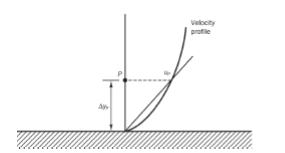
\includegraphics[width=0.5\linewidth]{fig/screenshot031}
\end{figure}
In
both cases the near wall flow is taken to be laminar it is assumed that the velocity varies
linearly with distance from the wall in a laminar flow. \newline 

When $y^+> 11.63$ node P is considered to be in the log law region of a
turbulent boundary layer, in
this region wall function formulae associated with the log law are used to calculate shear
stress, heat flux and other variables. 

\paragraph*{Moving walls} \mbox{} \\
Wall
movement in the x direction is felt by the fluid by a change in the wall shear stress: its value
is adjusted by replacing the absolute velocity by the relative velocity.

\subsection*{Constant Pressure}
The
constant pressure condition is used in situations where exact details of the flow distribution
are unknown but the boundary values of pressure are known. \newline 

A
convenient way of dealing with a constant pressure boundary condition is to fix pressure at the
nodes just inside the physical boundary. \newline

The
main problem is the unknown flow direction, which is governed by the conditions inside the
calculation domain

\subsection*{Symmetry}

The
conditions at a symmetry boundary are i no flow across the boundary and no scalar flux
across the boundary. \newline 

In
the implementation, normal velocities are set to zero at a symmetry boundary, and the values
of all other properties just outside the solution domain are equated to their values
at the nearest node just inside the domain. 

\subsection*{Final remarks}
Flows
inside a CFD solution domain are driven by the boundary conditions. In a certain way the process
of solving a fluid flow problem is nothing more than the extrapolation of a set of data defined on
a boundary contour or surface into the domain interior. 

It
is, therefore, of paramount importance that we supply physically realistic, well posed
boundary conditions, otherwise severe difficulties are encountered in obtaining solutions. \newline 

Particular
care must be taken in applying the outlet boundary condition: physically
the exit pressures govern the flow split between multiple outlets so it is better to
specify this quantity at exits than (zero gradient) outlet conditions. \newline 

It
is \textbf{not permitted} to combine an outlet condition with one or more constant pressure
boundaries, because the zero gradient outlet condition specifies neither the flow rate nor the
pressure at the exit, thus leaving the problem under specified. \newline 

If
outlet boundaries are placed too close to solid obstacles it is possible that the flow has not yet
reached a fully developed state (zero gradients in the flow direction), which may lead to errors.
	\begin{figure}[H]
		\centering
		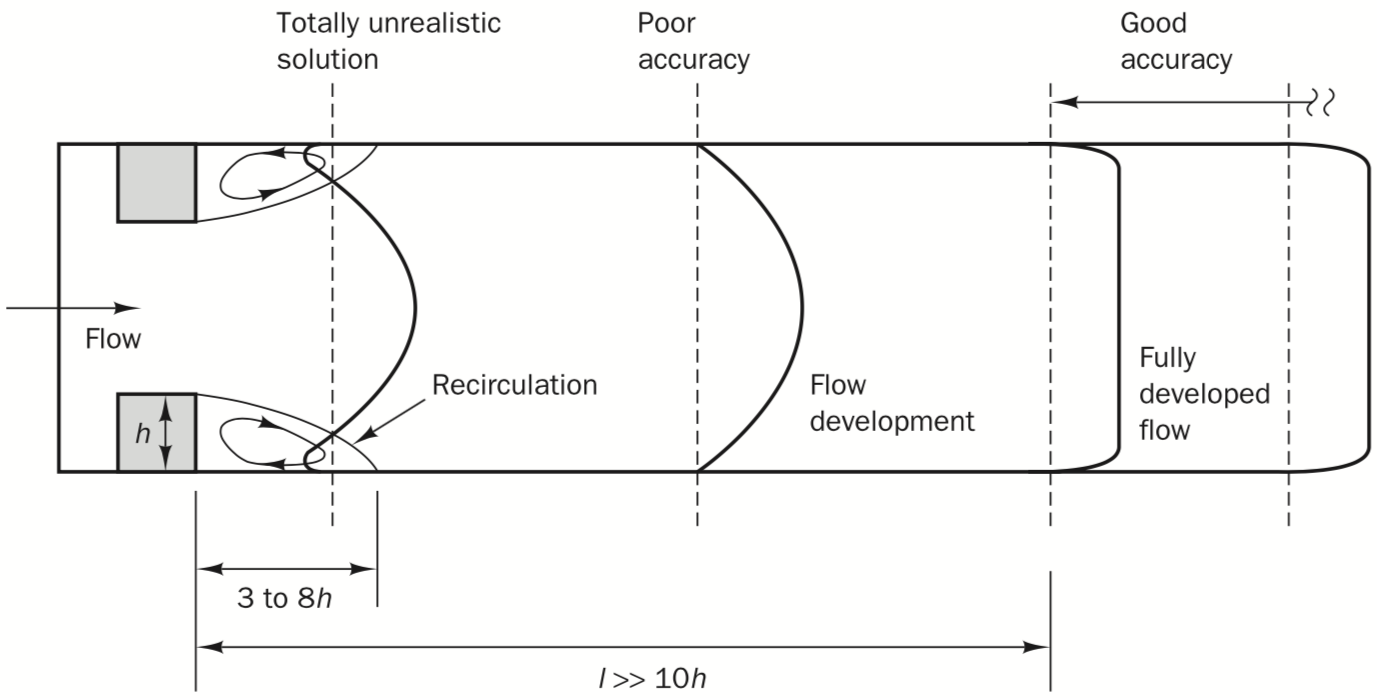
\includegraphics[width=0.5\linewidth]{fig/screenshot032}
		\label{fig:screenshot032}
	\end{figure}
It
is imperative that the outlet boundary is placed much further downstream than 10 heights of
the last obstacle to give accurate results. \newline 

For
high accuracy it is necessary to demonstrate that the interior solution is unaffected by the
choice of location of the outlet by means of a sensitivity study for the effect of different
downstream distances. 	
\end{document}
